\documentclass[]{article}
\usepackage[T1]{fontenc}
\usepackage{lmodern}
\usepackage{amssymb,amsmath}
\usepackage{ifxetex,ifluatex}
\usepackage{fixltx2e} % provides \textsubscript
% use upquote if available, for straight quotes in verbatim environments
\IfFileExists{upquote.sty}{\usepackage{upquote}}{}
\ifnum 0\ifxetex 1\fi\ifluatex 1\fi=0 % if pdftex
  \usepackage[utf8]{inputenc}
\else % if luatex or xelatex
  \ifxetex
    \usepackage{mathspec}
    \usepackage{xltxtra,xunicode}
  \else
    \usepackage{fontspec}
  \fi
  \defaultfontfeatures{Mapping=tex-text,Scale=MatchLowercase}
  \newcommand{\euro}{€}
\fi
% use microtype if available
\IfFileExists{microtype.sty}{\usepackage{microtype}}{}
\usepackage{longtable,booktabs}
\usepackage{graphicx}
% Redefine \includegraphics so that, unless explicit options are
% given, the image width will not exceed the width of the page.
% Images get their normal width if they fit onto the page, but
% are scaled down if they would overflow the margins.
\makeatletter
\def\ScaleIfNeeded{%
  \ifdim\Gin@nat@width>\linewidth
    \linewidth
  \else
    \Gin@nat@width
  \fi
}
\makeatother
\let\Oldincludegraphics\includegraphics
{%
 \catcode`\@=11\relax%
 \gdef\includegraphics{\@ifnextchar[{\Oldincludegraphics}{\Oldincludegraphics[width=\ScaleIfNeeded]}}%
}%
\ifxetex
  \usepackage[setpagesize=false, % page size defined by xetex
              unicode=false, % unicode breaks when used with xetex
              xetex]{hyperref}
\else
  \usepackage[unicode=true]{hyperref}
\fi
\hypersetup{breaklinks=true,
            bookmarks=true,
            pdfauthor={},
            pdftitle={},
            colorlinks=true,
            citecolor=blue,
            urlcolor=blue,
            linkcolor=magenta,
            pdfborder={0 0 0}}
\urlstyle{same}  % don't use monospace font for urls
\setlength{\parindent}{0pt}
\setlength{\parskip}{6pt plus 2pt minus 1pt}
\setlength{\emergencystretch}{3em}  % prevent overfull lines
\setcounter{secnumdepth}{0}
\usepackage{fancyhdr}
\pagestyle{fancy}
\lhead{C-Lyrics - A Word Cloud for Lyrics}
\rhead{\thepage}
\cfoot{Team 6}
\renewcommand{\headrulewidth}{0.4pt}
\renewcommand{\footrulewidth}{0.4pt}

\title{Clyrics - A Word Cloud for Lyrics}
\author{Justine Cocchi\\jcocchi@usc.edu \and Kelsey Fargas\\kfargas@usc.edu \and Mark Krant \\ mkrant@usc.edu\and Milad Gueramian\\gueramia@usc.edu \and Jeff Kang\\kangjr@usc.edu \and Séb Arnold\\arnolds@usc.edu}
\date{2 February 2015}

\title{%
	C-lyrics - A Word Cloud for Lyrics \\
	\large Software Project Management Plan}
    
\begin{document}

\maketitle

\pagebreak

\tableofcontents
\setcounter{tocdepth}{4}

\pagebreak

\section{Executive Summary}\label{executive-summary}

C-lyrics is a public website that will generate a word cloud for any given artist based on the 250 most frequently used words that appear across all of the artist’s published songs. This product will interface with the EchoNest API which will serve as the database from which we find and analyze the songs. By clicking on a specific word in the word cloud the user can see a list of all of the songs that word appears in and how frequently it occurs in each song. Furthermore, the user can click on any listed song title to see the complete lyrics for that song with the original word selected from the word cloud highlighted every time it appears. 

C-lyrics is intended for use by the general public. There will be no login required and there is no stored history of previous searches. Because of this we will have very low memory requirements and can run the product off of one server. The user can access C-lyrics using any device running any OS. After typing in the artist name and selecting the submit button, the word cloud will be generated in approximately one second and will be able to be shared via Facebook. 

\pagebreak

\section{1. Introduction}\label{introduction}

\subsection{1.1 Project Overview}\label{project-overview}

The primary objective of this project is to better understand the
software development lifecycle. For this specific project the objective
is to create a software system that allows a user to search for an
artist of their choice and generate a word cloud containing the most
popular used words from their lyrics database. This program will be
called C-lyrics, and is tentatively set to be delivered and readily
available for public use by March 11, 2015.

There are three major milestones that will be completed and have
subsections under each. These milestones consist of the completion of
all requirements set for each interface page, such as the home page,
songs page, and lyrics page. More details on these milestones can be
read in section 4.2. The master schedule will include five phases of
product development. These phases include designing the user interface,
implementing each function within the interfaces, testing these
interfaces, adding finishing touches, checking with the client, and
submitting. A more detailed Gantt chart will be located in section 4.1
and a more detailed description of costs can be found in section 3.

By completion, contributing members of this project should be able to
fully understand a product lifecycle as well as carrying out a complete
deliverable to all stakeholders.

\subsection{1.2 Project Deliverables}\label{project-deliverables}

The contributing authors to this documentation are the members of the
development team. They will create a fully functioning software program
that will allow anyone to specify any artist and generate a word cloud
comprised of that artist's most frequently used words. This software
program will also have the functionality to list the specified artist's
songs containing any word from the generated word cloud, and will allow
the user to select one of these listed songs to display its lyrics. This
program will be delivered as a product called C-lyrics. The client shall
receive all documentation associated with the product as well as
complete access and control of the product itself on March 11, 2015 at
THH 208 and on Blackboard. Only a single copy of each deliverable shall
be provided. These deliverables shall include software deliverables and
document deliverables. The software deliverables will include a working
software that will satisfy all set requirements and specifications made
at the beginning the project, and delivered online through Blackboard.
Document deliverables will include this current document as well as past
and previous documents to completely satisfy the clients' request.

\subsection{1.3 Evolution of the SPMP}\label{evolution-of-the-spmp}

The SPMP for C-lyrics will be available under a version control tool,
GIT, monitored by all contributing members, so any changes will be made
to the plan itself. The clients will be updated when significant changes
have been made to the prototype. The client and development team will be
able to access the updated document.

\subsection{1.4 Reference Materials}\label{reference-materials}

{[}1{]} IEEE. IEEE Std 830-1998 IEEE Recommended Practice for Software
Requirements Specifications. IEEE Computer Society, 1998.

{[}2{]} ``word cloud''.
\href{http://www.oxforddictionaries.com/us/definition/american_english/word-cloud}{Oxforddictionaries.com}
(January 31, 2015)

{[}3{]} EchoNest API
\href{http://developer.echonest.com/docs/v4/index.html\#overview}{documentation.}
(January 29, 2015)

{[}4{]} Van Vliet, Hans. Software Engineering: Principles and Practice.
3rd ed. Indianapolis, Indiana: Wiley, 2008. 170-71.

\subsection{1.5 Definitions and
Acronyms}\label{definitions-and-acronyms}

\begin{longtable}[c]{@{}ll@{}}
\toprule\addlinespace
\begin{minipage}[t]{0.47\columnwidth}\raggedright
Term
\end{minipage} & \begin{minipage}[t]{0.47\columnwidth}\raggedright
Definition
\end{minipage}
\\
\hline
\\\addlinespace
\begin{minipage}[t]{0.47\columnwidth}\raggedright
AJAX
\end{minipage} & \begin{minipage}[t]{0.47\columnwidth}\raggedright
Asynchronous JavaScript And XML. Technology allowing the transfer of
data from between the front- and back-end without reloading the web
page.
\end{minipage}
\\\addlinespace
\begin{minipage}[t]{0.47\columnwidth}\raggedright
API (EchoNest)
\end{minipage} & \begin{minipage}[t]{0.47\columnwidth}\raggedright
API will refer to the EchoNest API. EchoNest is a free API that allows
developers to retrieve lyrics and artist information in web pages and
other programs.
\end{minipage}
\\\addlinespace
\begin{minipage}[t]{0.47\columnwidth}\raggedright
Autocomplete
\end{minipage} & \begin{minipage}[t]{0.47\columnwidth}\raggedright
Autocomplete refers to the functionality addition to the Search Bar,
allowing users to enter minimal characters and choose artists that are
most similar to the string and display a picture of those artists next
to their name.
\end{minipage}
\\\addlinespace
\begin{minipage}[t]{0.47\columnwidth}\raggedright
Autocomplete Delay
\end{minipage} & \begin{minipage}[t]{0.47\columnwidth}\raggedright
A feature designed for the search bar when a user is typing. The delay
refers to the suspending action while the user is typing, making the
request to the server for autocomplete.
\end{minipage}
\\\addlinespace
\begin{minipage}[t]{0.47\columnwidth}\raggedright
Backend
\end{minipage} & \begin{minipage}[t]{0.47\columnwidth}\raggedright
References the PHP backend page
\end{minipage}
\\\addlinespace
\begin{minipage}[t]{0.47\columnwidth}\raggedright
Back to home button
\end{minipage} & \begin{minipage}[t]{0.47\columnwidth}\raggedright
A button redirecting the user to the homepage.
\end{minipage}
\\\addlinespace
\begin{minipage}[t]{0.47\columnwidth}\raggedright
Back to songs button
\end{minipage} & \begin{minipage}[t]{0.47\columnwidth}\raggedright
A button redirecting the user to the songs list page.
\end{minipage}
\\\addlinespace
\begin{minipage}[t]{0.47\columnwidth}\raggedright
Commonly Used Web Browser
\end{minipage} & \begin{minipage}[t]{0.47\columnwidth}\raggedright
Browsers such as Firefox, Safari, Chrome, Explorer, and Quora which come
on mobile phones, tablets and personal computers.
\end{minipage}
\\\addlinespace
\begin{minipage}[t]{0.47\columnwidth}\raggedright
Customer/Client
\end{minipage} & \begin{minipage}[t]{0.47\columnwidth}\raggedright
Dr. William G. Halfond and Sonal Mahajan
\end{minipage}
\\\addlinespace
\begin{minipage}[t]{0.47\columnwidth}\raggedright
GitHub
\end{minipage} & \begin{minipage}[t]{0.47\columnwidth}\raggedright
A web service that provides software version control tools.
www.github.com
\end{minipage}
\\\addlinespace
\begin{minipage}[t]{0.47\columnwidth}\raggedright
Stakeholders
\end{minipage} & \begin{minipage}[t]{0.47\columnwidth}\raggedright
The client and the development team
\end{minipage}
\\\addlinespace
\begin{minipage}[t]{0.47\columnwidth}\raggedright
LOC
\end{minipage} & \begin{minipage}[t]{0.47\columnwidth}\raggedright
acronym: for Lines of Code
\end{minipage}
\\\addlinespace
\begin{minipage}[t]{0.47\columnwidth}\raggedright
KSLOC
\end{minipage} & \begin{minipage}[t]{0.47\columnwidth}\raggedright
a metric that stands for: 1,000(K) Source Lines of Code
\end{minipage}
\\\addlinespace
\begin{minipage}[t]{0.47\columnwidth}\raggedright
Desktop Platform
\end{minipage} & \begin{minipage}[t]{0.47\columnwidth}\raggedright
A screen whose width exceeds 560px
\end{minipage}
\\\addlinespace
\begin{minipage}[t]{0.47\columnwidth}\raggedright
Development Team
\end{minipage} & \begin{minipage}[t]{0.47\columnwidth}\raggedright
All of the individuals whose names appear on the cover of this document.
These persons have collectively put this document together and will
collectively implement the software product described in subsequent
sections.
\end{minipage}
\\\addlinespace
\begin{minipage}[t]{0.47\columnwidth}\raggedright
Facebook
\end{minipage} & \begin{minipage}[t]{0.47\columnwidth}\raggedright
Online social network service where the generated word cloud image may
be shared amongst users.
\end{minipage}
\\\addlinespace
\begin{minipage}[t]{0.47\columnwidth}\raggedright
Google Doc
\end{minipage} & \begin{minipage}[t]{0.47\columnwidth}\raggedright
An online service provided by Google Inc. where an editable document~can
be accessed and change simultaneously by the members who have been given
access to the document. In the case of the development team, google doc
is the shared resource which contains the source of this SRS document.
\end{minipage}
\\\addlinespace
\begin{minipage}[t]{0.47\columnwidth}\raggedright
Home Page
\end{minipage} & \begin{minipage}[t]{0.47\columnwidth}\raggedright
The first page of the website visited by the user. It contains the Word
Cloud as well as the Search Bar.
\end{minipage}
\\\addlinespace
\begin{minipage}[t]{0.47\columnwidth}\raggedright
Lyrics Page
\end{minipage} & \begin{minipage}[t]{0.47\columnwidth}\raggedright
The third page of the website, it contains the lyrics for one song,
which is chosen by the user on the Songs Page. It will have two
Navigation Buttons that can take the user to either the Home Page or
back to the Songs Page.
\end{minipage}
\\\addlinespace
\begin{minipage}[t]{0.47\columnwidth}\raggedright
Mobile Platform
\end{minipage} & \begin{minipage}[t]{0.47\columnwidth}\raggedright
A screen whose width is less than or equal to 560px
\end{minipage}
\\\addlinespace
\begin{minipage}[t]{0.47\columnwidth}\raggedright
Navigation Buttons
\end{minipage} & \begin{minipage}[t]{0.47\columnwidth}\raggedright
Refers to any button that takes the user to previously visited pages of
the website.
\end{minipage}
\\\addlinespace
\begin{minipage}[t]{0.47\columnwidth}\raggedright
Software Project Management Plan (SPMP)
\end{minipage} & \begin{minipage}[t]{0.47\columnwidth}\raggedright
Refers to this document.
\end{minipage}
\\\addlinespace
\begin{minipage}[t]{0.47\columnwidth}\raggedright
Prototype
\end{minipage} & \begin{minipage}[t]{0.47\columnwidth}\raggedright
A small prototype of the software including the barebones of the
graphical display. Used during the second meeting with the client,
screenshots available in the appendices.
\end{minipage}
\\\addlinespace
\begin{minipage}[t]{0.47\columnwidth}\raggedright
Search Bar
\end{minipage} & \begin{minipage}[t]{0.47\columnwidth}\raggedright
The initial search bar on the first page of the website. Here, users can
type in artist or band names to generate a word cloud.
\end{minipage}
\\\addlinespace
\begin{minipage}[t]{0.47\columnwidth}\raggedright
Share Button
\end{minipage} & \begin{minipage}[t]{0.47\columnwidth}\raggedright
The standard, embeddable Facebook share button.
\end{minipage}
\\\addlinespace
\begin{minipage}[t]{0.47\columnwidth}\raggedright
Software or Product
\end{minipage} & \begin{minipage}[t]{0.47\columnwidth}\raggedright
The application software delivered from the supplier to the customer.
\end{minipage}
\\\addlinespace
\begin{minipage}[t]{0.47\columnwidth}\raggedright
Song List
\end{minipage} & \begin{minipage}[t]{0.47\columnwidth}\raggedright
This will be the culmination of all songs found that contain the search
word indicated by the user.
\end{minipage}
\\\addlinespace
\begin{minipage}[t]{0.47\columnwidth}\raggedright
Songs Page
\end{minipage} & \begin{minipage}[t]{0.47\columnwidth}\raggedright
The second page of the website. It contains the Song List as well as a
Navigation Button back to the Home Page. The user navigates to the Songs
page by clicking on a word in the Word Cloud on the Home page.
\end{minipage}
\\\addlinespace
\begin{minipage}[t]{0.47\columnwidth}\raggedright
Submit Button
\end{minipage} & \begin{minipage}[t]{0.47\columnwidth}\raggedright
The button adjacent to the Search Bar. When the user enters an artist
name into the Search Bar and is ready to generate the Word Cloud, he or
she must click on the Submit Button to begin the process.
\end{minipage}
\\\addlinespace
\begin{minipage}[t]{0.47\columnwidth}\raggedright
Supplier
\end{minipage} & \begin{minipage}[t]{0.47\columnwidth}\raggedright
The team developing the product for the customer.
\end{minipage}
\\\addlinespace
\begin{minipage}[t]{0.47\columnwidth}\raggedright
System
\end{minipage} & \begin{minipage}[t]{0.47\columnwidth}\raggedright
The set of machines running the software making it accessible to the
user.
\end{minipage}
\\\addlinespace
\begin{minipage}[t]{0.47\columnwidth}\raggedright
User
\end{minipage} & \begin{minipage}[t]{0.47\columnwidth}\raggedright
A person who interacts with C-lyrics software
\end{minipage}
\\\addlinespace
\begin{minipage}[t]{0.47\columnwidth}\raggedright
Word Cloud (WC)
\end{minipage} & \begin{minipage}[t]{0.47\columnwidth}\raggedright
A word cloud (otherwise known as a tag cloud) is, according to the
Oxford Dictionary, an image composed of words used in a particular text
or subject, in which the size of each word indicates its frequency or
importance {[}2{]}.
\end{minipage}
\\\addlinespace
\bottomrule
\end{longtable}

\section{2. Process and Organization}\label{process-and-organization}

\subsection{2.1 Software Lifecycle
Process}\label{software-lifecycle-process}

The software lifecycle process for this project will be based on the
Waterfall Model. In this model, each phase of software development needs
to be completed before attempting to work on the next phase. Testing is
the last phase of the process which takes place after the software has
been implemented.

\subsection{2.2 Team Organization}\label{team-organization}

The organizational structure of our team is flat with no specified
leader or hierarchy. Our team is structured by collaboration across all
members resulting in group decisions on who will work on each part of
the overall project. All internal deadlines and deliverables are set as
a team and communicated to everyone during team meetings and emails.
Each member of the team is equally responsible for every finished
deliverable as there is no team lead for any specific component.

\subsubsection{2.2.1 Current Group Process}\label{current-group-process}

The current group process in place for the development team is to meet
as an entire group whenever it is deemed necessary by a general
consensus. The consensus is gathered by means of group text messaging.
At each meeting, the development team decides the tasks to be completed,
progress made as of the time of the meeting and delegates future tasks
to each member for completion. This process has proved itself highly
effective as of the date of this publication and it is closely estimated
to continue through the entire life cycle of the software development
process for C-lyrics.

\subsubsection{2.2.2 Staff and Personnel
Plan}\label{staff-and-personnel-plan}

The C-Lyrics team will consist of the members of the development team.
Each member is proficient in object oriented design and concepts, and
has some familiarity with web development. Knowledge of git and other
version control methods is a must. The duration of need will be until
the last milestone and deliverable is reached. Each member will be
assigned tasks based on his or her prior knowledge. Since there will be
no training, members will have to research on the job if they are
insufficiently prepared. Personnel will not be phased out and retention
will not be a factor.

\subsubsection{2.2.3 Staff Allocation}\label{staff-allocation}

See \emph{Figure 1} for a detailed view of the staff allocation.

\begin{figure}[htbp]
\centering
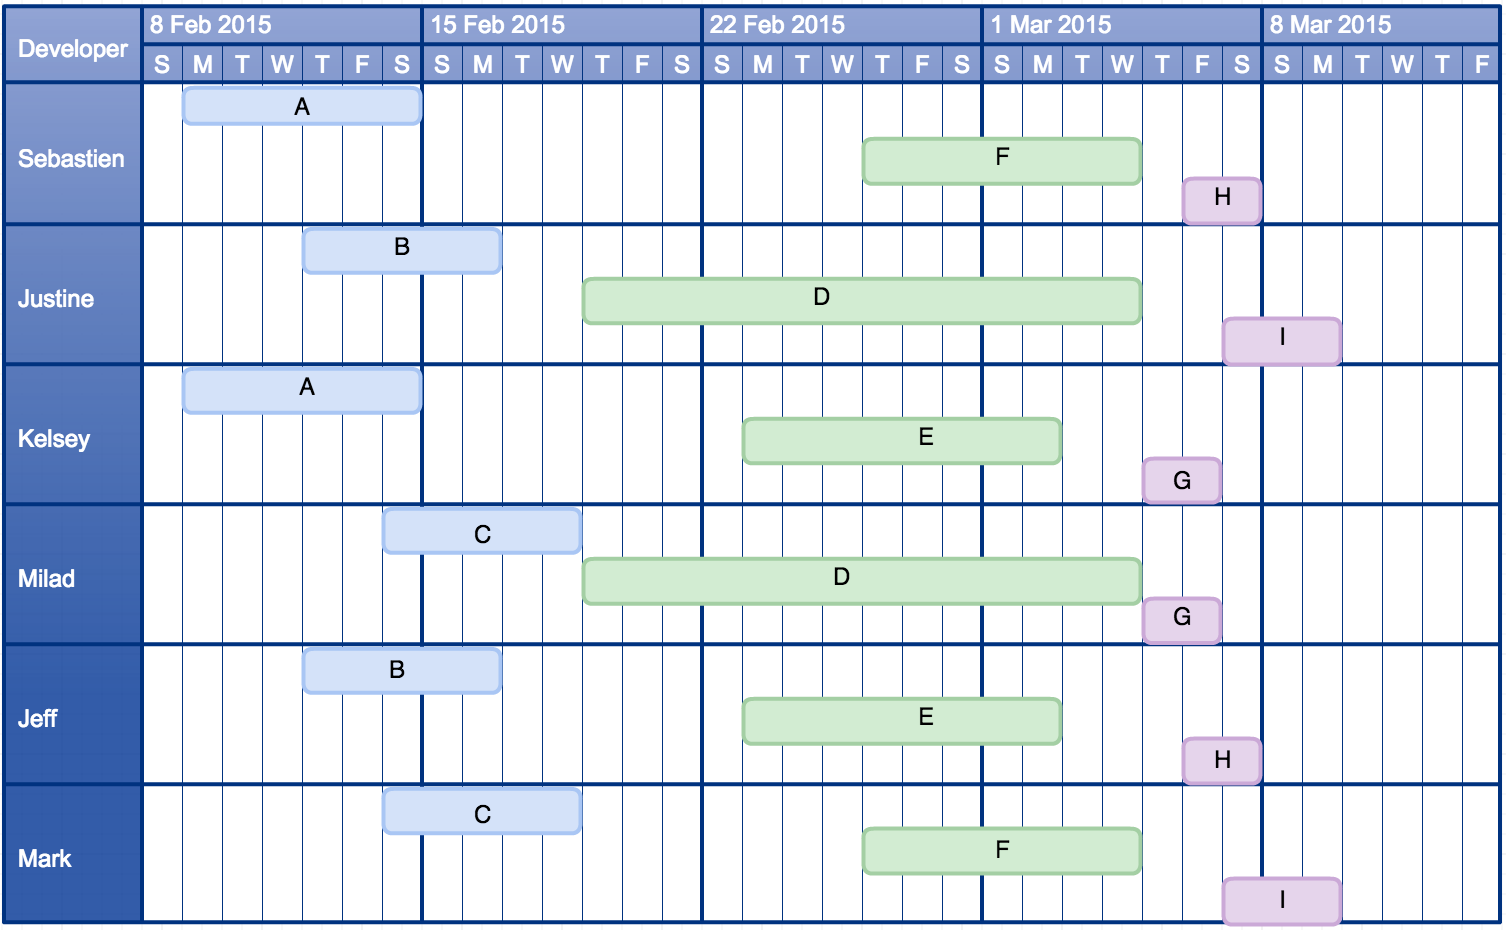
\includegraphics{StaffAllocation.png}
\caption{Staff Allocation}
\end{figure}

\subsubsection{2.2.4 Team Member
Description}\label{team-member-description}

This section provides a brief description of the members of the
development team and their relative experiences. Each member is a
student at the University of Southern California and is affiliated with
the Viterbi School of Engineering Computer Science Department. For
additional information on each member, refer to appendix for resumes.

\section{3. Cost Estimation}\label{cost-estimation}

\subsection{3.1 Cost Influence}\label{cost-influence}

The cost influencing factors that have been considered follow the
standard COCOMO II model for estimating project effort. These include
the four main categories of product factors, platform factors, personnel
factors, and project factors. The detailed list of cost drivers and the
associated estimations can be found in section 3.3 of this document.

\subsection{3.2 Cost Schedule
Relationship}\label{cost-schedule-relationship}

Cost and schedule are related based on the fact that this particular
project contains no defined wages in terms of fiscal costs. Therefore,
the only real ``cost'' is the effort and time that will be put into
creating the C-lyrics project. In other words, the schedule is perfectly
correlated with the cost of the project.

\subsection{3.3 Development Costs}\label{development-costs}

Our development costs have been estimated using the COCOMO II Model. The
following results are estimates of the cost drivers that are applied to
the model {[}4{]}.


\begin{center}
\textbf{Product Factors} \\
{
\centering
\begin{tabular}{ p{4cm} | p{4cm} }
Criteria & Value \\
\hline
Reliability required & very low, 0.75 \\
Database size & low, 0.93\\
Product complexity & low, 0.88 \\
Required reusability & nominal, 1.00\\
Documentation needs & very high, 1.13\\
\end{tabular}
}
\end{center}

The project requires very low reliability, since it would only pose a
slight inconvenience if the C-lyrics platform encountered problems and
was not available. We will most likely not need a database since the
lyrics generation will be based on an online API, therefore the database
size is listed as low. The low product complexity was selected based on
an average of the nominal control operations level and the very low
computational operations level. The reuse of components in the product
is nominal, since components only need to be reused within the project.
The documentation relative to the complexity of our project is very
high.


\begin{center}
\textbf{Platform Factors} \\
{
\centering
\begin{tabular}{ p{4cm} | p{4cm} }
Criteria & Value \\
\hline
Execution-time constraints & nominal, 1.0 \\
Main storage constraints & nominal, 1.0\\
Platform volatility & low, 0.87\\
\end{tabular}
}
\end{center}

The execution-time constraints are nominal since we will require less
than 50\% of available execution time. The main storage constraints are
nominal since we will require less than 50\% of available system
storage. Platform volatility is low since the hardware and software
required to run our program will not need frequent updates.

\begin{center}
\textbf{Personnel Factors} \\
{
\centering
\begin{tabular}{ p{4cm} | p{4cm} }
Criteria & Value \\
\hline
Analyst capability & very low, 1.50 \\
Programmer capability & low, 1.16 \\
Application experience & very low, 1.22 \\
Platform experience & low, 1.10 \\
Language and tool experience & low, 1.12 \\
Personnel continuity & very high, 0.84 \\
\end{tabular}
}
\end{center}

Analyst capability is very low since the group's ability to create
detailed, high-level design for software projects is minimal. Programmer
capability is low because of the lack of significant industry
programming experience of the team. Language and tool experience is low
since most of the team's programming experience centers around one or
two functional languages and little experience with software tools.
Personnel continuity is very high since all members of the team will
continue to be working together over the course of the project.

\begin{center}
\textbf{Project Factors} \\
{
\centering
\begin{tabular}{ p{4cm} | p{4cm} }
Criteria & Value \\
\hline
Use of software tools & low, 1.12 \\
Multi-site development & very high, 0.84 \\
Required development schedule & very high, 1.0 \\
\end{tabular}
}
\end{center}

The use of software tools is designated as low because we will not be
using highly developed tools that are structured for the purposes of our
project. The multi-site development rating is very high, since the group
has consistent communication both in person and through electronic
channels. The required development schedule is listed as very high since
the implementation phase of our project exceeds 160\% of the expected
time to complete the project.

The effort in terms of person-months is calculated as the KSLOC
multiplied by the product of all cost drivers according to COCOMO II.
With an estimated KSLOC of 1, the number of person-months that this
calculation returns is 1.247.

\subsection{3.4 External Costs}\label{external-costs}

Some of the external costs that are not directly factored into the
project costs include: purchasing the class textbook for research,
programming resources, and transportation costs for group incured by
individual members for meetings.

\section{4. Schedule, Milestones, and
Deliverables}\label{schedule-milestones-and-deliverables}

\subsection{4.1 Schedule}\label{schedule}

See \emph{Figure 2} for a detailed view of the staff allocation.

\begin{figure}[htbp]
\centering
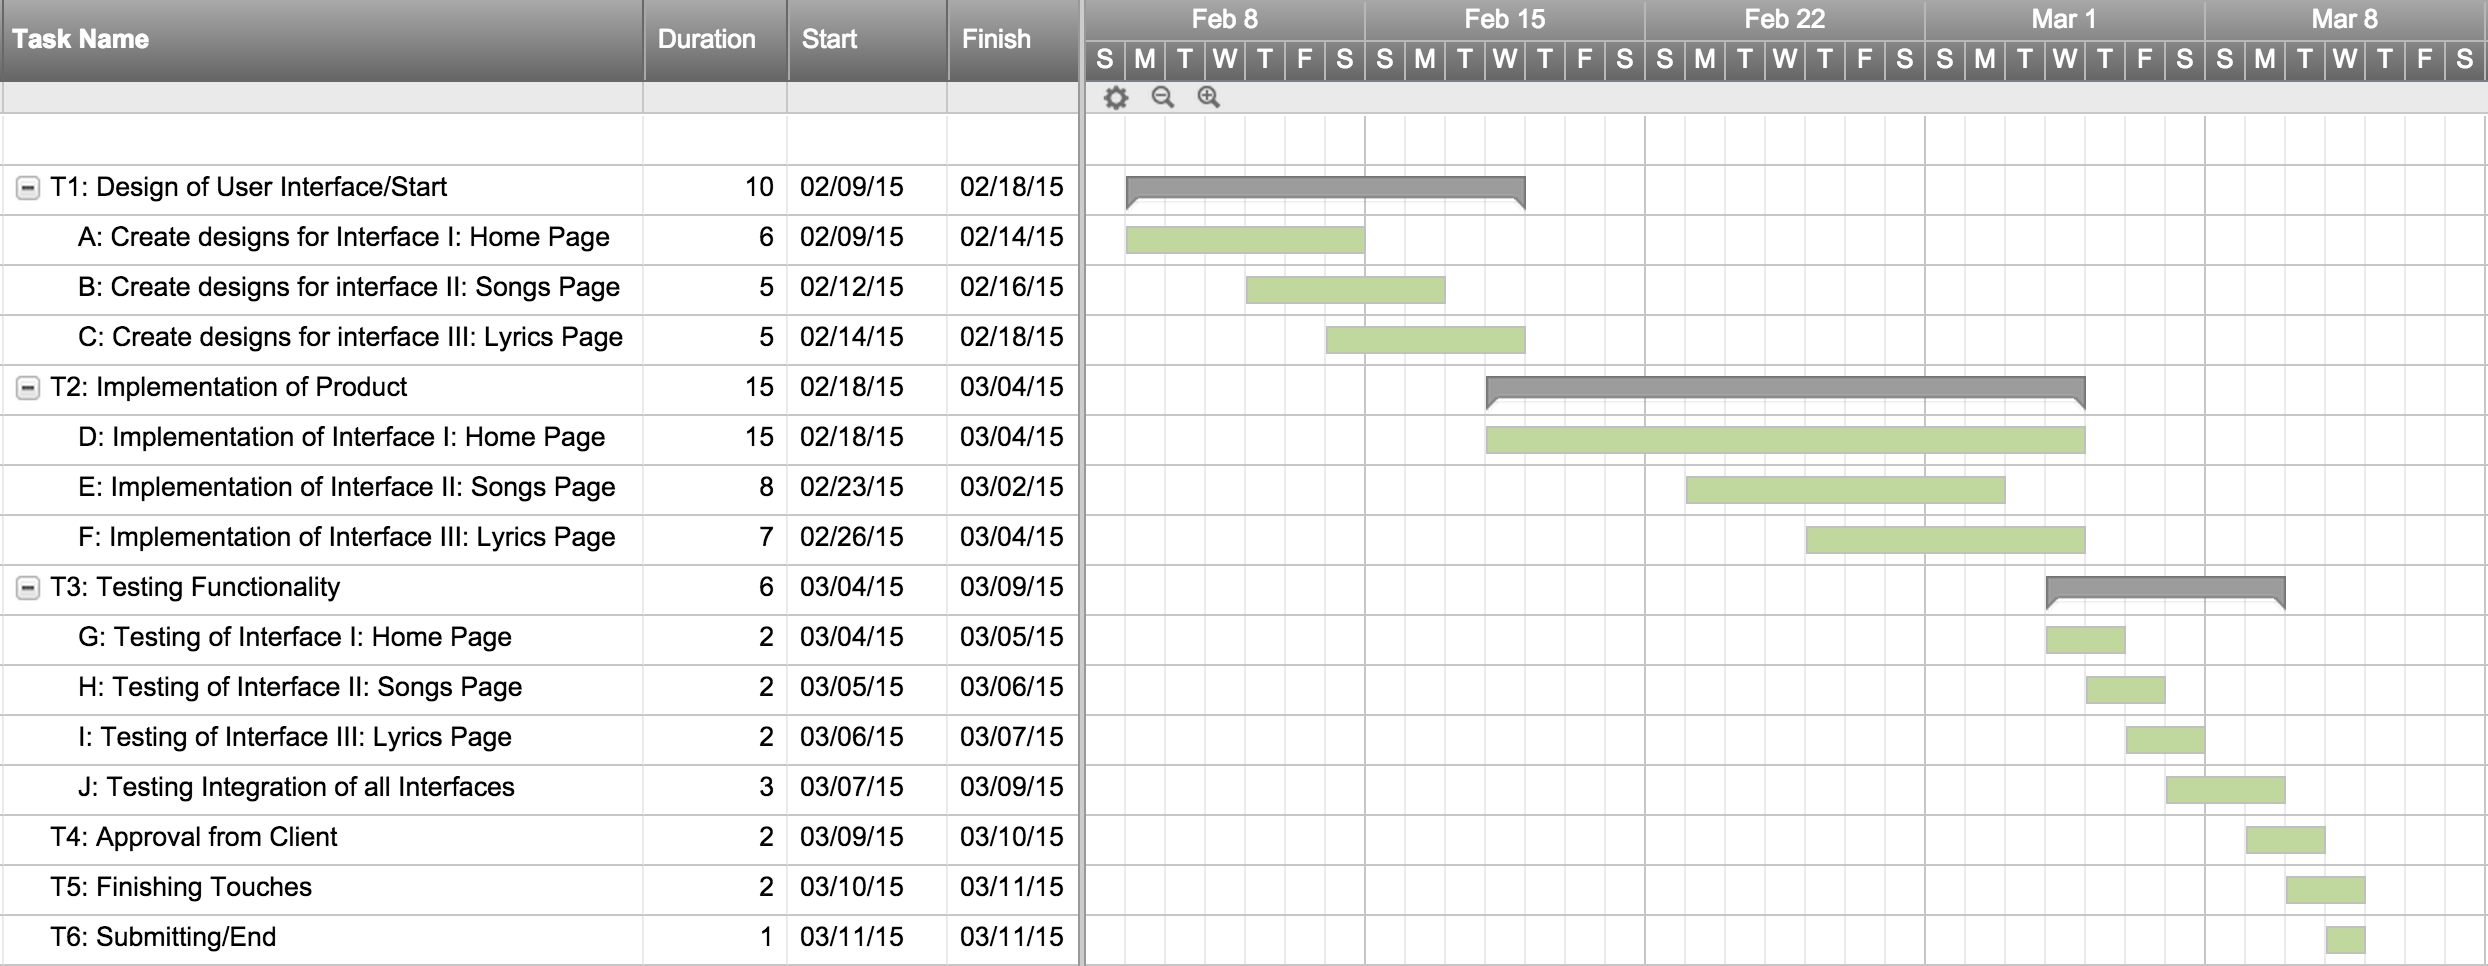
\includegraphics{schedule.png}
\caption{Schedule}
\end{figure}

\subsection{4.1.1 Activity Network}\label{activity-network}

See \emph{Figure 3} for a detailed view of the staff allocation, and
section 4.2 for the specific task encompassed in each milestone.

\begin{figure}[htbp]
\centering
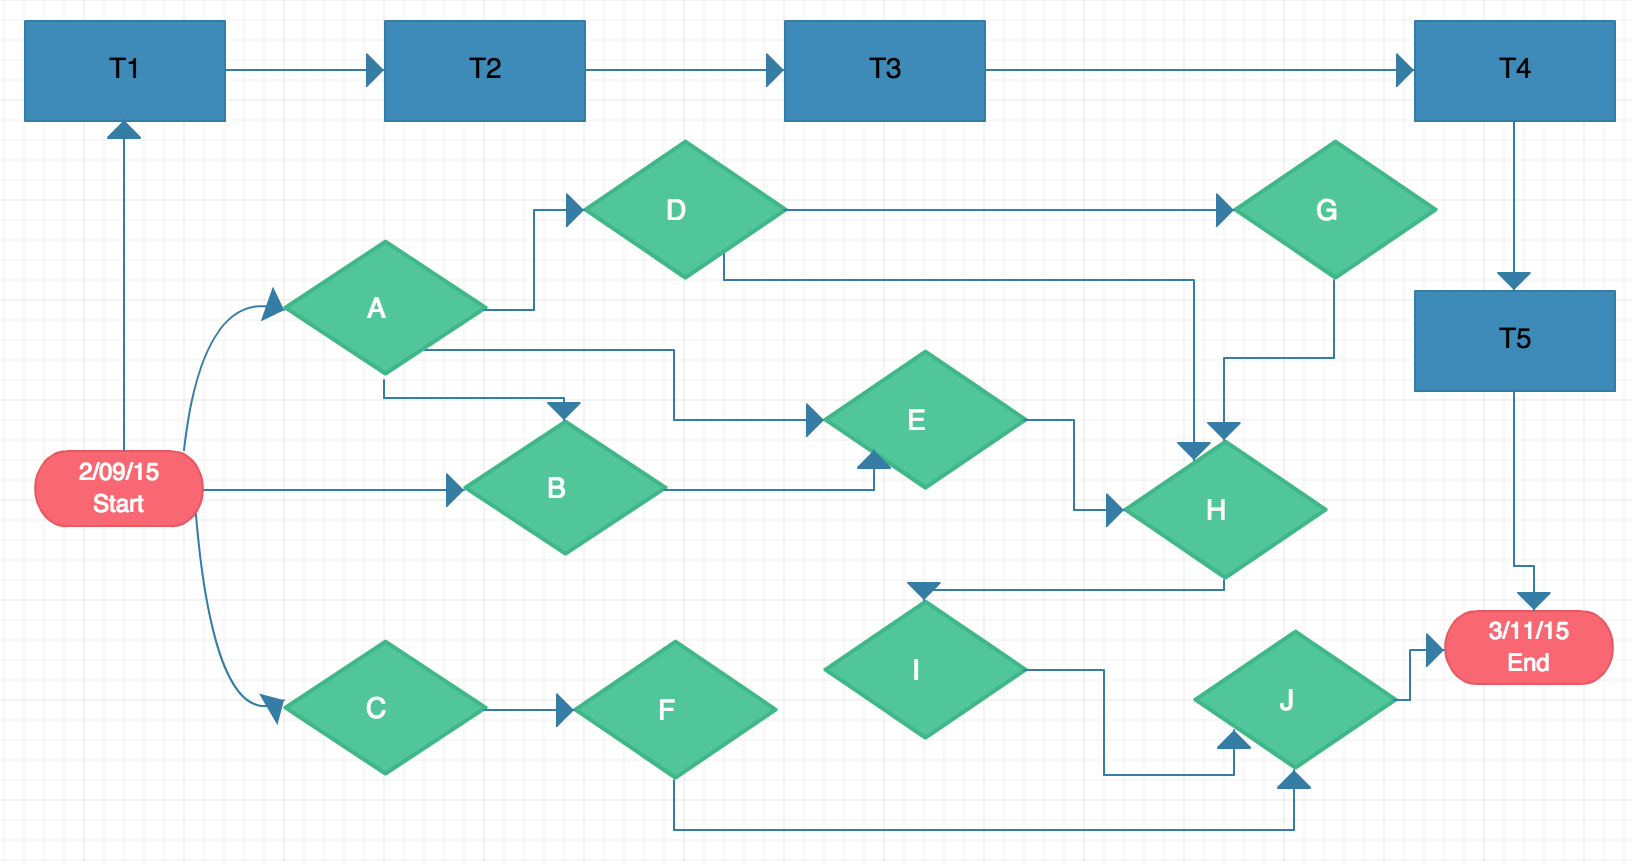
\includegraphics{ActivityNetwork.png}
\caption{Activity Network}
\end{figure}

\subsection{4.2 Project Milestones and
Deliverables}\label{project-milestones-and-deliverables}

The process model for our project is the Waterfall Model, meaning we
will finish each big software development phase before we start the
next. We will finish requirements engineering before starting the
project design, which will be finished before we start implementation,
which will be finished before we start testing, which will be finished
before we arrive at the final phase of project, maintenance.

Our project initiation was being assigned this project by Dr.~Halfond.
The first step in this project was beginning to work on the Software
Requirements Specification. The subsequent milestones and deliverables
are listed below.

Deliverables and Milestones:

\begin{itemize}
\itemsep1pt\parskip0pt\parsep0pt
\item
  Project Management
  Plan
  \ldots{}\ldots{}\ldots{}\ldots{}\ldots{}\ldots{}\ldots{}\ldots{}\ldots{}\ldots{}\ldots{}\ldots{}\ldots{}
  2/9/15
\item
  There are no specific milestones for this deliverable as it will be
  worked on by all team members and completed in full by February 9th.
\item
  Design\ldots{}\ldots{}\ldots{}\ldots{}\ldots{}\ldots{}\ldots{}\ldots{}\ldots{}\ldots{}\ldots{}\ldots{}\ldots{}\ldots{}\ldots{}\ldots{}\ldots{}\ldots{}\ldots{}2/18/15*
\item
  Milestones A-C

  \begin{itemize}
  \itemsep1pt\parskip0pt\parsep0pt
  \item
    A: Design of the Home Page

    \begin{itemize}
    \itemsep1pt\parskip0pt\parsep0pt
    \item
      A.1: Search bar
    \item
      A.2: WC generation
    \item
      A.3: Share button
    \item
      A.4: Add to Cloud
    \end{itemize}
  \item
    B: Design of the Songs Page

    \begin{itemize}
    \itemsep1pt\parskip0pt\parsep0pt
    \item
      B.1: List of songs
    \item
      B.2: Back to Home button
    \end{itemize}
  \item
    C: Design of the Lyrics Page

    \begin{itemize}
    \itemsep1pt\parskip0pt\parsep0pt
    \item
      C.1: Lyrics displayed on page
    \item
      C.2: Back to Songs button
    \item
      C.3: Back to Home button
    \end{itemize}
  \end{itemize}
\item
  Implementation\ldots{}\ldots{}\ldots{}\ldots{}\ldots{}\ldots{}\ldots{}\ldots{}\ldots{}\ldots{}\ldots{}\ldots{}\ldots{}\ldots{}\ldots{}\ldots{}..3/4/15*
\item
  Milestones D-F

  \begin{itemize}
  \itemsep1pt\parskip0pt\parsep0pt
  \item
    D: Implementation of the Home Page

    \begin{itemize}
    \itemsep1pt\parskip0pt\parsep0pt
    \item
      D.1: Search bar with autocomplete functionality when typing in an
      artist's name
    \item
      D.2: WC generation with words that can be selected to take the
      user to the Songs Page
    \item
      D.3: Share button to upload the WC to Facebook
    \item
      D.4: Add to Cloud button to create a new WC based off of words
      commonly used by both of the specified artists
    \end{itemize}
  \item
    E: Implementation of the Songs Page

    \begin{itemize}
    \itemsep1pt\parskip0pt\parsep0pt
    \item
      E.1: List of songs sorted by how frequently the selected word is
      used in each song
    \item
      E.2: Song titles in list able to be selected, taking the user to
      the Lyrics page
    \item
      E.3: Back to Home button takes the user back to the Home Page with
      the WC still displayed and the artist's name still in the Search
      Bar
    \end{itemize}
  \item
    F: Implementation of the Lyrics Page

    \begin{itemize}
    \itemsep1pt\parskip0pt\parsep0pt
    \item
      F.1: Lyrics displayed on page with the selected word highlighted
      every time it appears in the song
    \item
      F.2: Back to Songs button takes the user back to the Songs Page
      with the same list of songs still displayed in the same order
    \item
      F.3: Back to Home button takes the user back to the Home Page with
      the WC still displayed and the artist's name still in the Search
      Bar
    \end{itemize}
  \end{itemize}
\item
  Testing and Final
  Delivery\ldots{}\ldots{}\ldots{}\ldots{}\ldots{}\ldots{}\ldots{}\ldots{}\ldots{}..\ldots{}\ldots{}\ldots{}\ldots{}3/11/15*
\item
  Milestones G-J

  \begin{itemize}
  \itemsep1pt\parskip0pt\parsep0pt
  \item
    G: Testing of the Home Page

    \begin{itemize}
    \itemsep1pt\parskip0pt\parsep0pt
    \item
      G.1: Search bar with autocomplete functionality when typing in an
      artist's name
    \item
      G.2: WC generation with words that can be selected to take the
      user to the Songs Page
    \item
      G.3: Share button to upload the WC to Facebook
    \item
      G.4: Add to Cloud button to create a new WC based off of words
      commonly used by both of the specified artists
    \end{itemize}
  \item
    H: Testing of the Songs Page

    \begin{itemize}
    \itemsep1pt\parskip0pt\parsep0pt
    \item
      H.1: List of songs sorted by how frequently the selected word is
      used in each song
    \item
      H.2: Song titles in list able to be selected, taking the user to
      the Lyrics page
    \item
      H.3: Back to Home button takes the user back to the Home Page with
      the WC still displayed and the artist's name still in the Search
      Bar
    \end{itemize}
  \item
    I: Testing of the Lyrics Page

    \begin{itemize}
    \itemsep1pt\parskip0pt\parsep0pt
    \item
      I.1: Lyrics displayed on page with the selected word highlighted
      every time it appears in the song
    \item
      I.2: Back to Songs button takes the user back to the Songs Page
      with the same list of songs still displayed in the same order
    \item
      I.3: Back to Home button takes the user back to the Home Page with
      the WC still displayed and the artist's name still in the Search
      Bar
    \end{itemize}
  \item
    J: Testing of the entire product to ensure all pages work together
    as specified in the SRS
  \end{itemize}
\end{itemize}

Deliverables with an asterisk (*) by the due date indicate that there
are risk factors that may alter the completion date. These risk factors
include, but are not limited to, changing requirements for each
deliverable and the deliverables taking either more or less time than
expected. Due dates for each milestone are listed in the schedule in
section 4.1. Also note that these dates are subject to change by the
client and are only tentative (dates are from project schedule given by
client, where it is noted that they are subject to change)

The termination activity of our project is presenting the completed
product to both Dr.~Halfond and Ms.~Mahajan and ensuring that both of
them are satisfied with our work. However, if this is not accomplished
by the final project deadline, 3/11/15, then our project will be
terminated regardless of the customer's satisfaction.

\section{5. Configuration Management
Plans}\label{configuration-management-plans}

\subsection{5.1 Product Documentation
Management}\label{product-documentation-management}

Formal report formats between the client and development team will be
structured according to IEEE standards and use LaTeX as a document
preparation system for the client. The code documentation will be
generated by Sphinx, which provides an easy way to create intelligent
and beautiful documentation. In particular, it allows the documentation
to be generated in several formats (eg, HTML, LaTeX, PDF) directly from
the comments in the source code. Therefore, the documentation will
partly be integrated in the code base and will be versioned by git as
well. These processes will be used for the Software Requirements
Specifications (SRS), Software Project Management Plan (SPMP), and a
Design Document (DD).

\subsection{5.2 Code Base Management}\label{code-base-management}

The whole code of the project will hosted and managed by the git
program. Specifically, the project is going to be divided in three main
repositories; the frontend, the backend and a third repository for
general purpose. All three of the repositories will be hosted by
GitHub.com and they will belong to the C-Lyrics organisation. This will
allow the development team to better coordinate their effort while
creating the software, and takes care of most of the merges in the code
base. As stated in Section 5.3, the GitHub repositories will be coupled
with Travis CI for continuous integration.

\subsection{5.3 Software Quality Assurance
Plan}\label{software-quality-assurance-plan}

Reviews and audits will take place after every milestone is completed.
The development team will review the progress made thus far to make sure
deadlines will be met, while observing and complying with the details of
the project management plan. If there are noticeable shortcomings and
deviations in the current progress of the project from what has been
decided in the project management plan, audits to the project will have
to be made.

In addition, the software will be developed according the Test Driven
Development methodology. This aims to provide an additional measure for
the advancement of the project as well as an assurance on its quality.
By writing the basic tests first and then implementing the functions so
that they pass the tests, the goal of the development process is
slightly modified. Instead of aiming to implement every requirement and
functionality, the objective is to have all the pre-written tests
pass.To keep track of such advancements, GitHub will be coupled with
Travis CI allowing continuous integration along the process. Finally
some code coverage tools (ie, JSCoverage, PHP\_Unit) will be used in
order to keep track of the percentage of total coverage on the project.

In order to keep track of the progress, the development team will use a
custom metric. Essentially, the metric mixes the objectivity of the test
coverage as well as the personal insights of the team members. Each team
member will give a grade from 1 to 5 to each one of the other members
based on the amount of work they accomplished. Each member's score will
be averaged and the average of these averages will be the final score of
the team. This score is then combined with the amount of tests that pass
as well as the amount of code coverage. Hopefully, this combination of
both an objective metric as well as the team's self opinion on how they
are doing provides an accurate estimation of the progress on the
project. The mathematical details and some additional reasons for the
use of this metric are included in the Appendix.

\subsection{5.4 Project Monitoring Plan}\label{project-monitoring-plan}

Github's issue tracker and progress reporting system, along with Google
Docs, will be used as the primary project monitoring mechanism among
team members. Tasks will be assigned to each team member with a
description and a project milestone. Each issue completion will
correspond to a milestone set in the project management plan. If there
is a change in the milestone contents and dates, the issue tracker will
be updated in accordance and strictly follow the most up to date plan.
Once the task is completed, the team member will submit the deliverables
to Github and mark the task in the issue tracker as completed.

\section{6. Risk Management Plan}\label{risk-management-plan}

\subsection{6.1 Risk Identification}\label{risk-identification}

\begin{longtable}[c]{@{}ll@{}}
\toprule\addlinespace
\begin{minipage}[t]{0.47\columnwidth}\raggedright
Risk Type
\end{minipage} & \begin{minipage}[t]{0.47\columnwidth}\raggedright
Possible Risks
\end{minipage}
\\\addlinespace
\begin{minipage}[t]{0.47\columnwidth}\raggedright
Technology
\end{minipage} & \begin{minipage}[t]{0.47\columnwidth}\raggedright
The maximum number of queries allowed on EchoNest is reached during
testing.

The server that is hosting the domain goes down.

The website traffic is overloaded, causing a crash.

The real-time performance of the software is inadequate.
\end{minipage}
\\\addlinespace
\begin{minipage}[t]{0.47\columnwidth}\raggedright
People
\end{minipage} & \begin{minipage}[t]{0.47\columnwidth}\raggedright
Staff members do not have the required technical skills demanded by the
project and must spend time to learn them.

One or more members of the staff are seriously ill or incapable of
working.

Staff members who lack experience are unable to learn quick enough to
meet deadlines.
\end{minipage}
\\\addlinespace
\begin{minipage}[t]{0.47\columnwidth}\raggedright
Organisational
\end{minipage} & \begin{minipage}[t]{0.47\columnwidth}\raggedright
One or more new staff members are added to the development team.

One or more of the current staff members quits.

A flat organization produces a lack of accountability and confusion,
resulting in delayed deliverables.

The waterfall method is ineffective due to changing customer demands and
uncertainties.
\end{minipage}
\\\addlinespace
\begin{minipage}[t]{0.47\columnwidth}\raggedright
Metrics
\end{minipage} & \begin{minipage}[t]{0.47\columnwidth}\raggedright
The metrics are not completely objective
\end{minipage}
\\\addlinespace
\begin{minipage}[t]{0.47\columnwidth}\raggedright
Tools
\end{minipage} & \begin{minipage}[t]{0.47\columnwidth}\raggedright
The chosen CASE tools cannot be integrated into the software without
serious restructuring.
\end{minipage}
\\\addlinespace
\begin{minipage}[t]{0.47\columnwidth}\raggedright
Requirements
\end{minipage} & \begin{minipage}[t]{0.47\columnwidth}\raggedright
The client and stakeholder want to alter small details of the product.

The client and stakeholder want to restructure the product entirely.

Requirements from the client are misinterpreted during implementation.

The development team implements features that looks aesthetically
pleasing, but is unwanted by the client.
\end{minipage}
\\\addlinespace
\begin{minipage}[t]{0.47\columnwidth}\raggedright
Estimation
\end{minipage} & \begin{minipage}[t]{0.47\columnwidth}\raggedright
The software takes longer to develop than previously anticipated.

The number of ~people using the software is greater than what was
previously decided by the client and stakeholder.
\end{minipage}
\\\addlinespace
\bottomrule
\end{longtable}

\subsection{6.2 Risk Analysis}\label{risk-analysis}

\begin{longtable}[c]{@{}llll@{}}
\toprule\addlinespace
\begin{minipage}[t]{0.22\columnwidth}\raggedright
No.
\end{minipage} & \begin{minipage}[t]{0.22\columnwidth}\raggedright
Risk
\end{minipage} & \begin{minipage}[t]{0.22\columnwidth}\raggedright
Probability
\end{minipage} & \begin{minipage}[t]{0.22\columnwidth}\raggedright
Effects
\end{minipage}
\\\addlinespace
\begin{minipage}[t]{0.22\columnwidth}\raggedright
1
\end{minipage} & \begin{minipage}[t]{0.22\columnwidth}\raggedright
The maximum number of queries allowed on EchoNest is reached during
testing.
\end{minipage} & \begin{minipage}[t]{0.22\columnwidth}\raggedright
Very Low
\end{minipage} & \begin{minipage}[t]{0.22\columnwidth}\raggedright
Catastrophic
\end{minipage}
\\\addlinespace
\begin{minipage}[t]{0.22\columnwidth}\raggedright
2
\end{minipage} & \begin{minipage}[t]{0.22\columnwidth}\raggedright
The server that is hosting the domain crashes.
\end{minipage} & \begin{minipage}[t]{0.22\columnwidth}\raggedright
Low
\end{minipage} & \begin{minipage}[t]{0.22\columnwidth}\raggedright
Serious
\end{minipage}
\\\addlinespace
\begin{minipage}[t]{0.22\columnwidth}\raggedright
3
\end{minipage} & \begin{minipage}[t]{0.22\columnwidth}\raggedright
The website traffic is overloaded, causing a crash.
\end{minipage} & \begin{minipage}[t]{0.22\columnwidth}\raggedright
Very Low
\end{minipage} & \begin{minipage}[t]{0.22\columnwidth}\raggedright
Serious
\end{minipage}
\\\addlinespace
\begin{minipage}[t]{0.22\columnwidth}\raggedright
4
\end{minipage} & \begin{minipage}[t]{0.22\columnwidth}\raggedright
Staff members do not have the required technical skills demanded by the
project and must spend time to learn them.
\end{minipage} & \begin{minipage}[t]{0.22\columnwidth}\raggedright
Moderate
\end{minipage} & \begin{minipage}[t]{0.22\columnwidth}\raggedright
Tolerable
\end{minipage}
\\\addlinespace
\begin{minipage}[t]{0.22\columnwidth}\raggedright
5
\end{minipage} & \begin{minipage}[t]{0.22\columnwidth}\raggedright
One or more members of the staff are seriously ill or incapable of
working.
\end{minipage} & \begin{minipage}[t]{0.22\columnwidth}\raggedright
Low
\end{minipage} & \begin{minipage}[t]{0.22\columnwidth}\raggedright
Serious
\end{minipage}
\\\addlinespace
\begin{minipage}[t]{0.22\columnwidth}\raggedright
6
\end{minipage} & \begin{minipage}[t]{0.22\columnwidth}\raggedright
Staff members who lack experience are unable to learn quick enough to
meet deadlines.
\end{minipage} & \begin{minipage}[t]{0.22\columnwidth}\raggedright
Low
\end{minipage} & \begin{minipage}[t]{0.22\columnwidth}\raggedright
Serious
\end{minipage}
\\\addlinespace
\begin{minipage}[t]{0.22\columnwidth}\raggedright
7
\end{minipage} & \begin{minipage}[t]{0.22\columnwidth}\raggedright
One or more new staff members are added to the development team.
\end{minipage} & \begin{minipage}[t]{0.22\columnwidth}\raggedright
Low
\end{minipage} & \begin{minipage}[t]{0.22\columnwidth}\raggedright
Insignificant
\end{minipage}
\\\addlinespace
\begin{minipage}[t]{0.22\columnwidth}\raggedright
8
\end{minipage} & \begin{minipage}[t]{0.22\columnwidth}\raggedright
One or more of the current staff members quits.
\end{minipage} & \begin{minipage}[t]{0.22\columnwidth}\raggedright
Low
\end{minipage} & \begin{minipage}[t]{0.22\columnwidth}\raggedright
Tolerable
\end{minipage}
\\\addlinespace
\begin{minipage}[t]{0.22\columnwidth}\raggedright
9
\end{minipage} & \begin{minipage}[t]{0.22\columnwidth}\raggedright
The chosen CASE tools cannot be integrated into the software without
serious restructuring.
\end{minipage} & \begin{minipage}[t]{0.22\columnwidth}\raggedright
Moderate
\end{minipage} & \begin{minipage}[t]{0.22\columnwidth}\raggedright
Tolerable
\end{minipage}
\\\addlinespace
\begin{minipage}[t]{0.22\columnwidth}\raggedright
10
\end{minipage} & \begin{minipage}[t]{0.22\columnwidth}\raggedright
The client and stakeholder request to alter small details of the
product.
\end{minipage} & \begin{minipage}[t]{0.22\columnwidth}\raggedright
High
\end{minipage} & \begin{minipage}[t]{0.22\columnwidth}\raggedright
Tolerable
\end{minipage}
\\\addlinespace
\begin{minipage}[t]{0.22\columnwidth}\raggedright
11
\end{minipage} & \begin{minipage}[t]{0.22\columnwidth}\raggedright
The client and stakeholder want to restructure the product entirely.
\end{minipage} & \begin{minipage}[t]{0.22\columnwidth}\raggedright
Moderate
\end{minipage} & \begin{minipage}[t]{0.22\columnwidth}\raggedright
Catastrophic
\end{minipage}
\\\addlinespace
\begin{minipage}[t]{0.22\columnwidth}\raggedright
12
\end{minipage} & \begin{minipage}[t]{0.22\columnwidth}\raggedright
The software takes longer to develop than previously anticipated.
\end{minipage} & \begin{minipage}[t]{0.22\columnwidth}\raggedright
High
\end{minipage} & \begin{minipage}[t]{0.22\columnwidth}\raggedright
Tolerable
\end{minipage}
\\\addlinespace
\begin{minipage}[t]{0.22\columnwidth}\raggedright
13
\end{minipage} & \begin{minipage}[t]{0.22\columnwidth}\raggedright
The number of users is greater than what was previously decided by the
client and stakeholder.
\end{minipage} & \begin{minipage}[t]{0.22\columnwidth}\raggedright
Moderate
\end{minipage} & \begin{minipage}[t]{0.22\columnwidth}\raggedright
Tolerable
\end{minipage}
\\\addlinespace
\begin{minipage}[t]{0.22\columnwidth}\raggedright
14
\end{minipage} & \begin{minipage}[t]{0.22\columnwidth}\raggedright
A flat organization produces a lack of accountability and confusion,
resulting in delayed deliverables.
\end{minipage} & \begin{minipage}[t]{0.22\columnwidth}\raggedright
Moderate
\end{minipage} & \begin{minipage}[t]{0.22\columnwidth}\raggedright
Serious
\end{minipage}
\\\addlinespace
\begin{minipage}[t]{0.22\columnwidth}\raggedright
15
\end{minipage} & \begin{minipage}[t]{0.22\columnwidth}\raggedright
The waterfall method is ineffective due to changing customer demands and
uncertainties.
\end{minipage} & \begin{minipage}[t]{0.22\columnwidth}\raggedright
Moderate
\end{minipage} & \begin{minipage}[t]{0.22\columnwidth}\raggedright
Tolerable
\end{minipage}
\\\addlinespace
\begin{minipage}[t]{0.22\columnwidth}\raggedright
16
\end{minipage} & \begin{minipage}[t]{0.22\columnwidth}\raggedright
The real-time performance of the software is inadequate.
\end{minipage} & \begin{minipage}[t]{0.22\columnwidth}\raggedright
Moderate
\end{minipage} & \begin{minipage}[t]{0.22\columnwidth}\raggedright
Serious
\end{minipage}
\\\addlinespace
\begin{minipage}[t]{0.22\columnwidth}\raggedright
17
\end{minipage} & \begin{minipage}[t]{0.22\columnwidth}\raggedright
Requirements from the client are misinterpreted during implementation.
\end{minipage} & \begin{minipage}[t]{0.22\columnwidth}\raggedright
High
\end{minipage} & \begin{minipage}[t]{0.22\columnwidth}\raggedright
Tolerable
\end{minipage}
\\\addlinespace
\begin{minipage}[t]{0.22\columnwidth}\raggedright
18
\end{minipage} & \begin{minipage}[t]{0.22\columnwidth}\raggedright
The development team implements features that looks aesthetically
pleasing, but is unwanted by the client.
\end{minipage} & \begin{minipage}[t]{0.22\columnwidth}\raggedright
Moderate
\end{minipage} & \begin{minipage}[t]{0.22\columnwidth}\raggedright
Tolerable
\end{minipage}
\\\addlinespace
\begin{minipage}[t]{0.22\columnwidth}\raggedright
19
\end{minipage} & \begin{minipage}[t]{0.22\columnwidth}\raggedright
Objectibility of custom metric to track progress of project is low
\end{minipage} & \begin{minipage}[t]{0.22\columnwidth}\raggedright
Moderate
\end{minipage} & \begin{minipage}[t]{0.22\columnwidth}\raggedright
Tolerable
\end{minipage}
\\\addlinespace
\bottomrule
\end{longtable}
\subsection{6.3 Risk Planning}\label{risk-planning}

\begin{longtable}[c]{@{}lll@{}}
\toprule\addlinespace
\begin{minipage}[t]{0.30\columnwidth}\raggedright
Risk No.
\end{minipage} & \begin{minipage}[t]{0.30\columnwidth}\raggedright
Strategy Type
\end{minipage} & \begin{minipage}[t]{0.30\columnwidth}\raggedright
Solution
\end{minipage}
\\\addlinespace
\begin{minipage}[t]{0.30\columnwidth}\raggedright
1
\end{minipage} & \begin{minipage}[t]{0.30\columnwidth}\raggedright
Avoidance
\end{minipage} & \begin{minipage}[t]{0.30\columnwidth}\raggedright
Make smarter test cases that cover more areas of vulnerability in a
smaller amount of API queries.
\end{minipage}
\\\addlinespace
\begin{minipage}[t]{0.30\columnwidth}\raggedright
2
\end{minipage} & \begin{minipage}[t]{0.30\columnwidth}\raggedright
Avoidance
\end{minipage} & \begin{minipage}[t]{0.30\columnwidth}\raggedright
Host the software on a reliable server, or perhaps change the hosting
location based off of previous crashing problems..
\end{minipage}
\\\addlinespace
\begin{minipage}[t]{0.30\columnwidth}\raggedright
3
\end{minipage} & \begin{minipage}[t]{0.30\columnwidth}\raggedright
Avoidance
\end{minipage} & \begin{minipage}[t]{0.30\columnwidth}\raggedright
Select a more robust hosting service.
\end{minipage}
\\\addlinespace
\begin{minipage}[t]{0.30\columnwidth}\raggedright
4
\end{minipage} & \begin{minipage}[t]{0.30\columnwidth}\raggedright
Contingency Plan
\end{minipage} & \begin{minipage}[t]{0.30\columnwidth}\raggedright
Allocate staff members to develop parts of the project that best suits
their skills. If no one is familiar with the language or practices
required, work in teams of two to promote collaboration
\end{minipage}
\\\addlinespace
\begin{minipage}[t]{0.30\columnwidth}\raggedright
5
\end{minipage} & \begin{minipage}[t]{0.30\columnwidth}\raggedright
Contingency Plan
\end{minipage} & \begin{minipage}[t]{0.30\columnwidth}\raggedright
Assign the tasks of the ill staff member to various other members, while
the ill staff member can update the new members on the current state of
the task.
\end{minipage}
\\\addlinespace
\begin{minipage}[t]{0.30\columnwidth}\raggedright
6
\end{minipage} & \begin{minipage}[t]{0.30\columnwidth}\raggedright
Contingency Plan
\end{minipage} & \begin{minipage}[t]{0.30\columnwidth}\raggedright
Delay the deliverable output, or submit the incomplete deliverable and
patch the mistakes later when given more time.
\end{minipage}
\\\addlinespace
\begin{minipage}[t]{0.30\columnwidth}\raggedright
7
\end{minipage} & \begin{minipage}[t]{0.30\columnwidth}\raggedright
Minimisation
\end{minipage} & \begin{minipage}[t]{0.30\columnwidth}\raggedright
Update the new staff member with the current state of the software and
introduce low level tasks to help get him or her up to speed.
\end{minipage}
\\\addlinespace
\begin{minipage}[t]{0.30\columnwidth}\raggedright
8
\end{minipage} & \begin{minipage}[t]{0.30\columnwidth}\raggedright
Minimisation
\end{minipage} & \begin{minipage}[t]{0.30\columnwidth}\raggedright
Allocate the work of the quitting staff member among the remaining team
members.
\end{minipage}
\\\addlinespace
\begin{minipage}[t]{0.30\columnwidth}\raggedright
9
\end{minipage} & \begin{minipage}[t]{0.30\columnwidth}\raggedright
Contingency Plan
\end{minipage} & \begin{minipage}[t]{0.30\columnwidth}\raggedright
Find new tools to fill the needs of the software.
\end{minipage}
\\\addlinespace
\begin{minipage}[t]{0.30\columnwidth}\raggedright
10
\end{minipage} & \begin{minipage}[t]{0.30\columnwidth}\raggedright
Contingency Plan
\end{minipage} & \begin{minipage}[t]{0.30\columnwidth}\raggedright
Update previous documents with the new information and fill out a
revision history of each document. Change the code to fit the demands
and, depending on the magnitude of the desired changes, restructuring of
the software may be necessary.
\end{minipage}
\\\addlinespace
\begin{minipage}[t]{0.30\columnwidth}\raggedright
11
\end{minipage} & \begin{minipage}[t]{0.30\columnwidth}\raggedright
Contingency Plan
\end{minipage} & \begin{minipage}[t]{0.30\columnwidth}\raggedright
Depending on the amount of change desired by the client, the staff may
have to create new documents entirely and essentially start a new
project.
\end{minipage}
\\\addlinespace
\begin{minipage}[t]{0.30\columnwidth}\raggedright
12
\end{minipage} & \begin{minipage}[t]{0.30\columnwidth}\raggedright
Contingency Plan
\end{minipage} & \begin{minipage}[t]{0.30\columnwidth}\raggedright
Change the deliverable dates to compensate for a new estimated time
using COCOMO.
\end{minipage}
\\\addlinespace
\begin{minipage}[t]{0.30\columnwidth}\raggedright
13
\end{minipage} & \begin{minipage}[t]{0.30\columnwidth}\raggedright
Minimisation
\end{minipage} & \begin{minipage}[t]{0.30\columnwidth}\raggedright
To compensate for more users than previously intended, the software may
have to be altered to more effectively handle storage, the EchoNest API
licensing may have to be purchased to allow more requests, and the
server will need to be able to handle more requests.
\end{minipage}
\\\addlinespace
\begin{minipage}[t]{0.30\columnwidth}\raggedright
14
\end{minipage} & \begin{minipage}[t]{0.30\columnwidth}\raggedright
Minimisation
\end{minipage} & \begin{minipage}[t]{0.30\columnwidth}\raggedright
Hold team members more accountable for his or her own tasks. Part of
this can be achieved by instilling a productive atmosphere during
meetings and other official work times. If there continues to be
problems with a flat organization, a hierarchy may need to be introduced
to inspire more efficient work.
\end{minipage}
\\\addlinespace
\begin{minipage}[t]{0.30\columnwidth}\raggedright
15
\end{minipage} & \begin{minipage}[t]{0.30\columnwidth}\raggedright
Contingency Plan
\end{minipage} & \begin{minipage}[t]{0.30\columnwidth}\raggedright
The development team will have to work around the inefficiencies of the
waterfall method. Switching to Agile methodology is not an option.
\end{minipage}
\\\addlinespace
\begin{minipage}[t]{0.30\columnwidth}\raggedright
16
\end{minipage} & \begin{minipage}[t]{0.30\columnwidth}\raggedright
Avoidance
\end{minipage} & \begin{minipage}[t]{0.30\columnwidth}\raggedright
The development team will need to structure the code in a way that
produces results in the quickest way possible. If it is too slow,
restructuring may be required. Caching results is one way to speed up
results.
\end{minipage}
\\\addlinespace
\begin{minipage}[t]{0.30\columnwidth}\raggedright
17
\end{minipage} & \begin{minipage}[t]{0.30\columnwidth}\raggedright
Avoidance
\end{minipage} & \begin{minipage}[t]{0.30\columnwidth}\raggedright
If the requirements specified by the client is different than what is
implemented, the development team will have to fix the unwanted
components. This can be avoided by following the requirements document
closely, assuming the client specified everything during the formation
of the requirements document.
\end{minipage}
\\\addlinespace
\begin{minipage}[t]{0.30\columnwidth}\raggedright
18
\end{minipage} & \begin{minipage}[t]{0.30\columnwidth}\raggedright
Avoidance
\end{minipage} & \begin{minipage}[t]{0.30\columnwidth}\raggedright
The development team should follow the requirements document regardless
of the opinions of the team on the specifications of components.
\end{minipage}
\\\addlinespace
\bottomrule
\end{longtable}

\subsection{6.4 Risk Monitoring}\label{risk-monitoring}

Throughout the development cycle, the team will have to monitor each
risk regularly and prepare for it depending on the estimated likelihood
that it will occur. Each member will be aware of the risk pertaining to
his or her tasks and discuss the chance that they occur at each meeting.
Many risks do not involve the actual implementation and cannot be
anticipated, therefore these risks can be ignored during team meetings.
Larger risks for a particular milestone or deliverable can be noted in
the github issue tracker along with the regular team meeting procedure.

\section{7. Appendices}\label{appendices}

\subsection{A.1: Appendix 1: Meetings with
Customer}\label{a.1-appendix-1-meetings-with-customer}

\subsubsection{Change to Requirements}\label{change-to-requirements}

\begin{itemize}
\itemsep1pt\parskip0pt\parsep0pt
\item
  On February 5, 2015, the client indicated a change in the text color
  preferences for the WC. Before, the client required the text color of
  the WC to be black. Now, there should be different, randomly assigned
  colors for each word.
\end{itemize}

\subsubsection{Added Details}\label{added-details}

\begin{itemize}
\itemsep1pt\parskip0pt\parsep0pt
\item
  Search bar should be user friendly, user should be able to leave out
  common words and still get an accurate suggestion.
\item
  Search bar should have some sort of direction for the user as to how
  he/she should proceed
\end{itemize}

\subsection{A.2: Appendix 2: Metric and
Measurement}\label{a.2-appendix-2-metric-and-measurement}

$$
$$


\subsection{A.3: Appendix 3: COCOMO
Details}\label{a.3-appendix-3-cocomo-details}

We used the COCOMO II model for estimating the work required to complete
our project because it is an effective standard formula that takes
initial assumptions and makes a useful projection from them. Although
the cost drivers operate based on assumed levels, we feel that the
calculation takes several important factors into account, making up for
any subjectivity. The individual assumptions for why we chose certain
levels for each driver is listed in section 3.3. We also made an
assumption for the KSLOC, estimating that our project will reach about
1,000 source lines of code. We are assuming that the project will be
rather small compared to industry software projects since the website
does not need to be excessively robust in design and functionality.

\subsubsection{Formula}\label{formula}

\[
E(person-months) = b \cdot KLOC^c
\] (our estimation for KLOC approx = 1)

\subsection{A.4: Appendix 4: Resumes}\label{a.4-appendix-4-resumes}
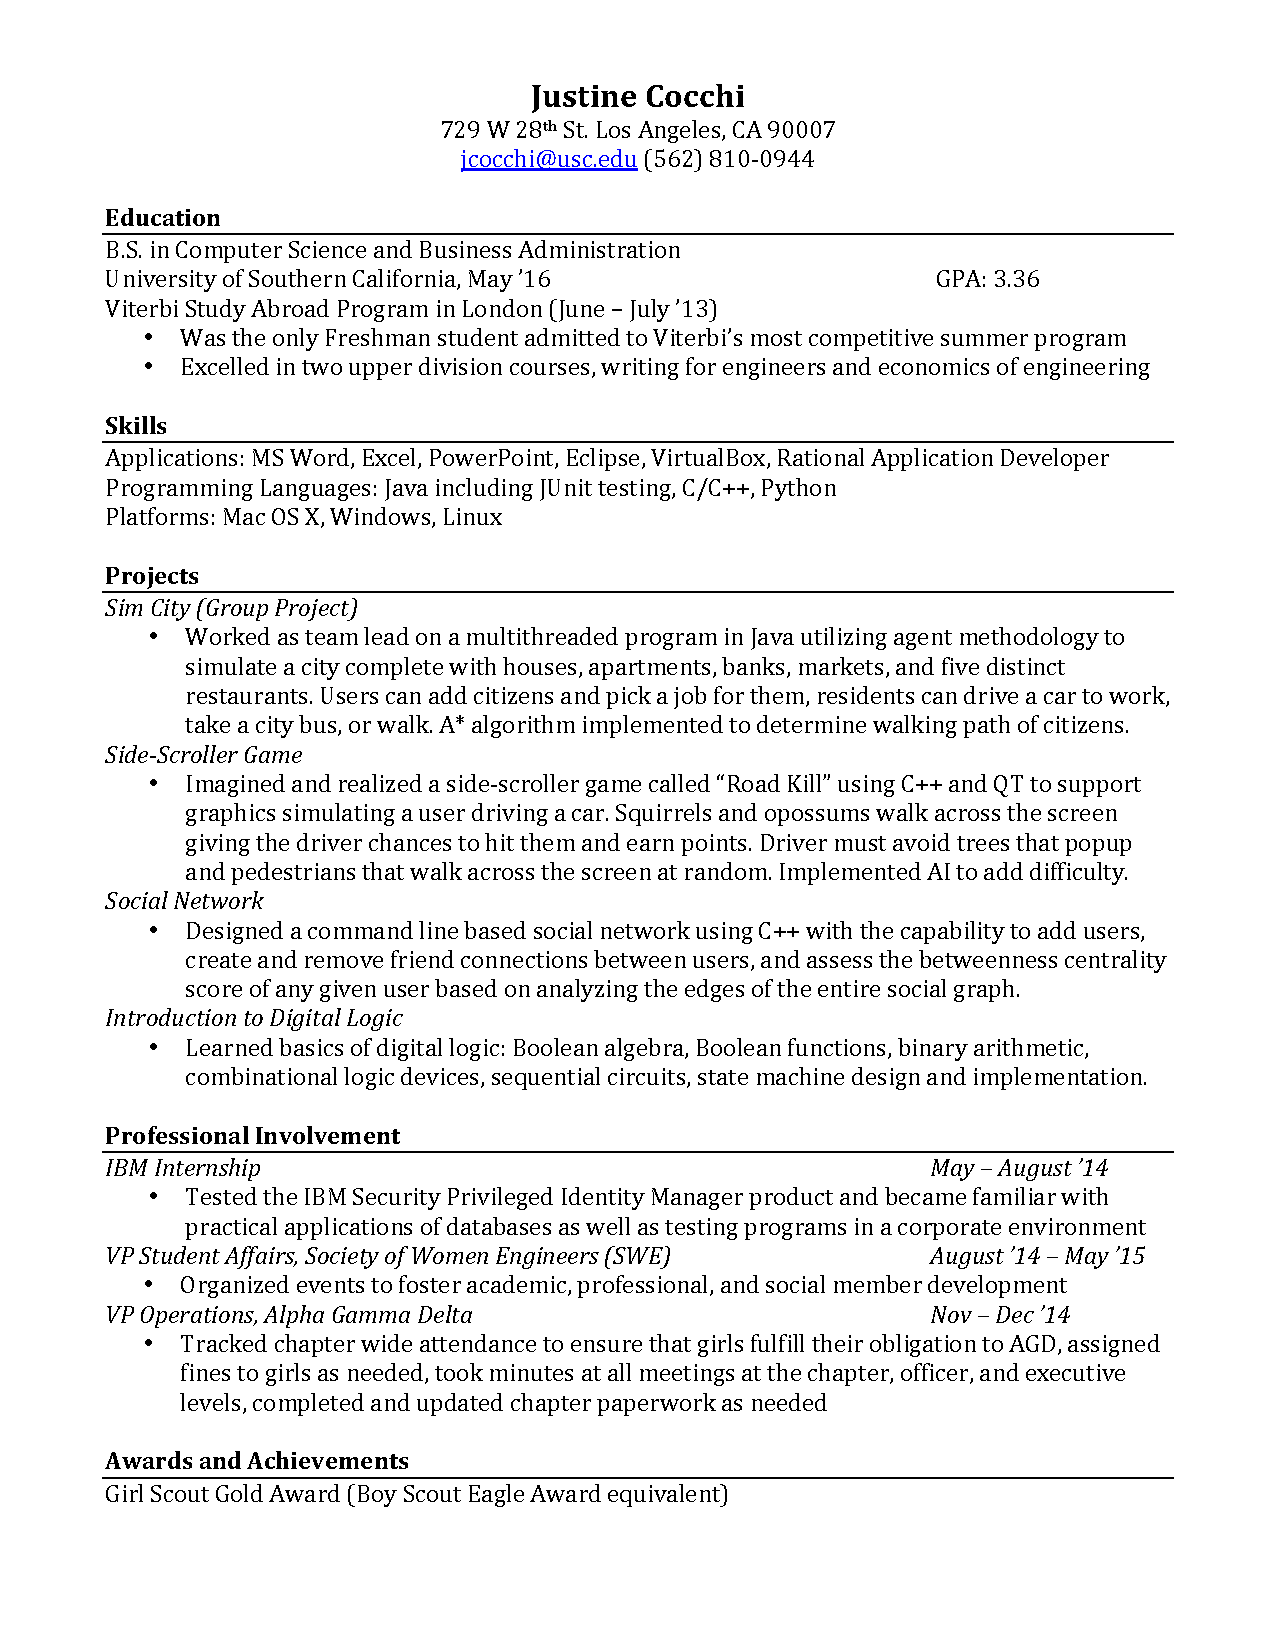
\includegraphics{justine.pdf}
\pagebreak

\pagebreak

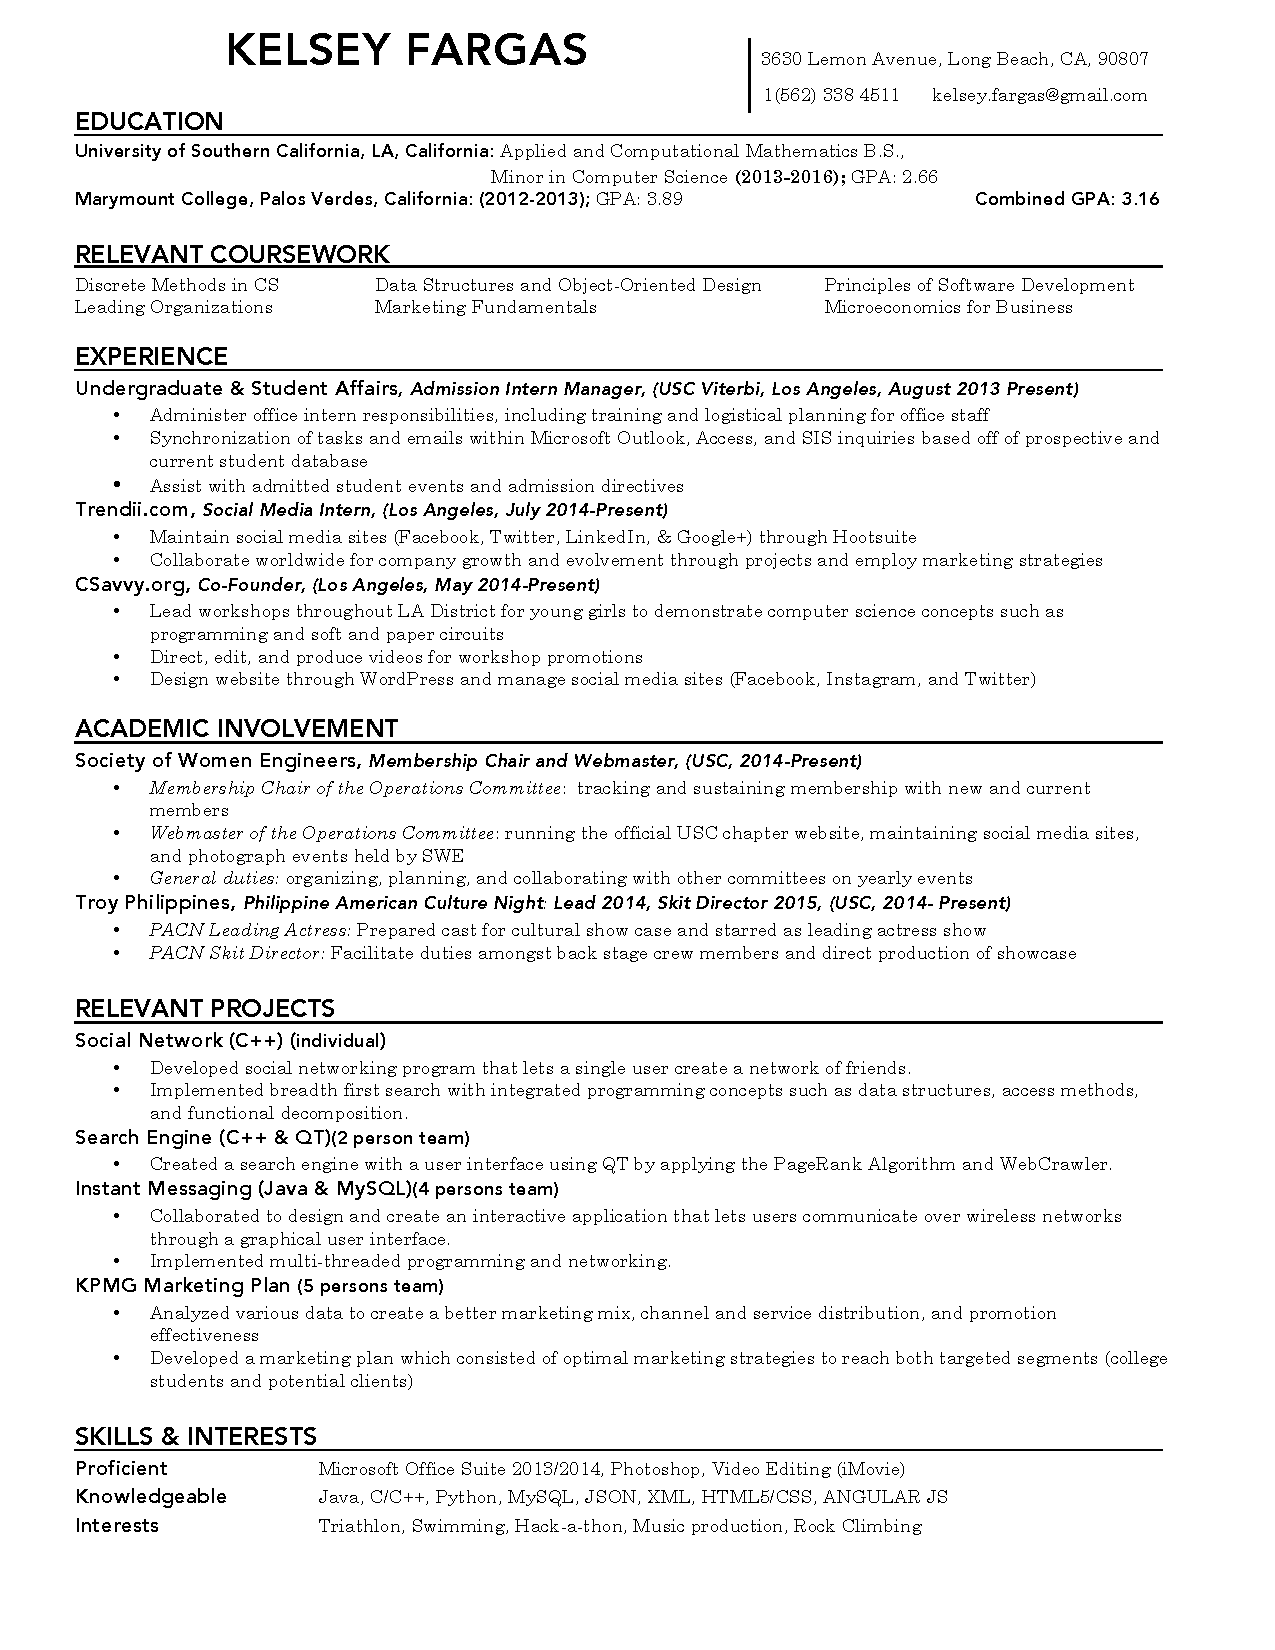
\includegraphics{kelsey.pdf}
\pagebreak

\pagebreak

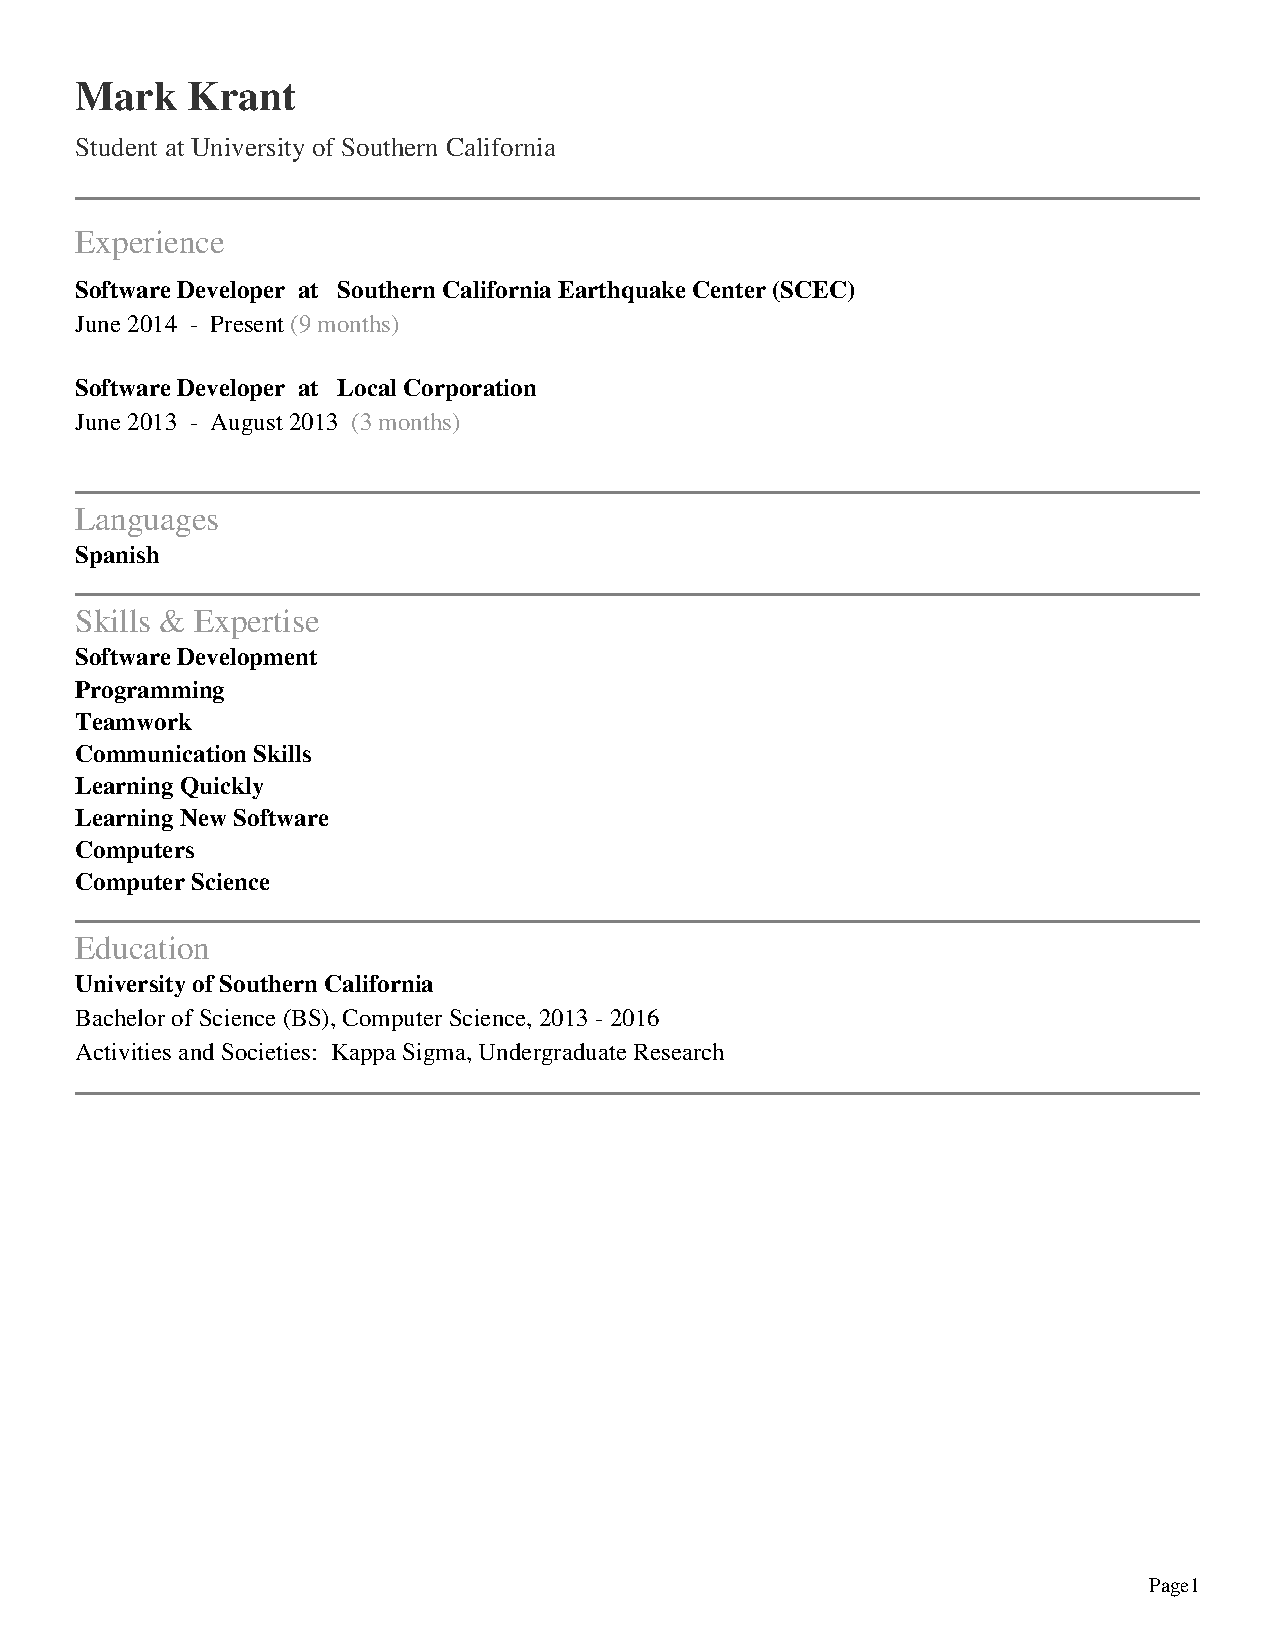
\includegraphics{mark.pdf}
\pagebreak

\pagebreak

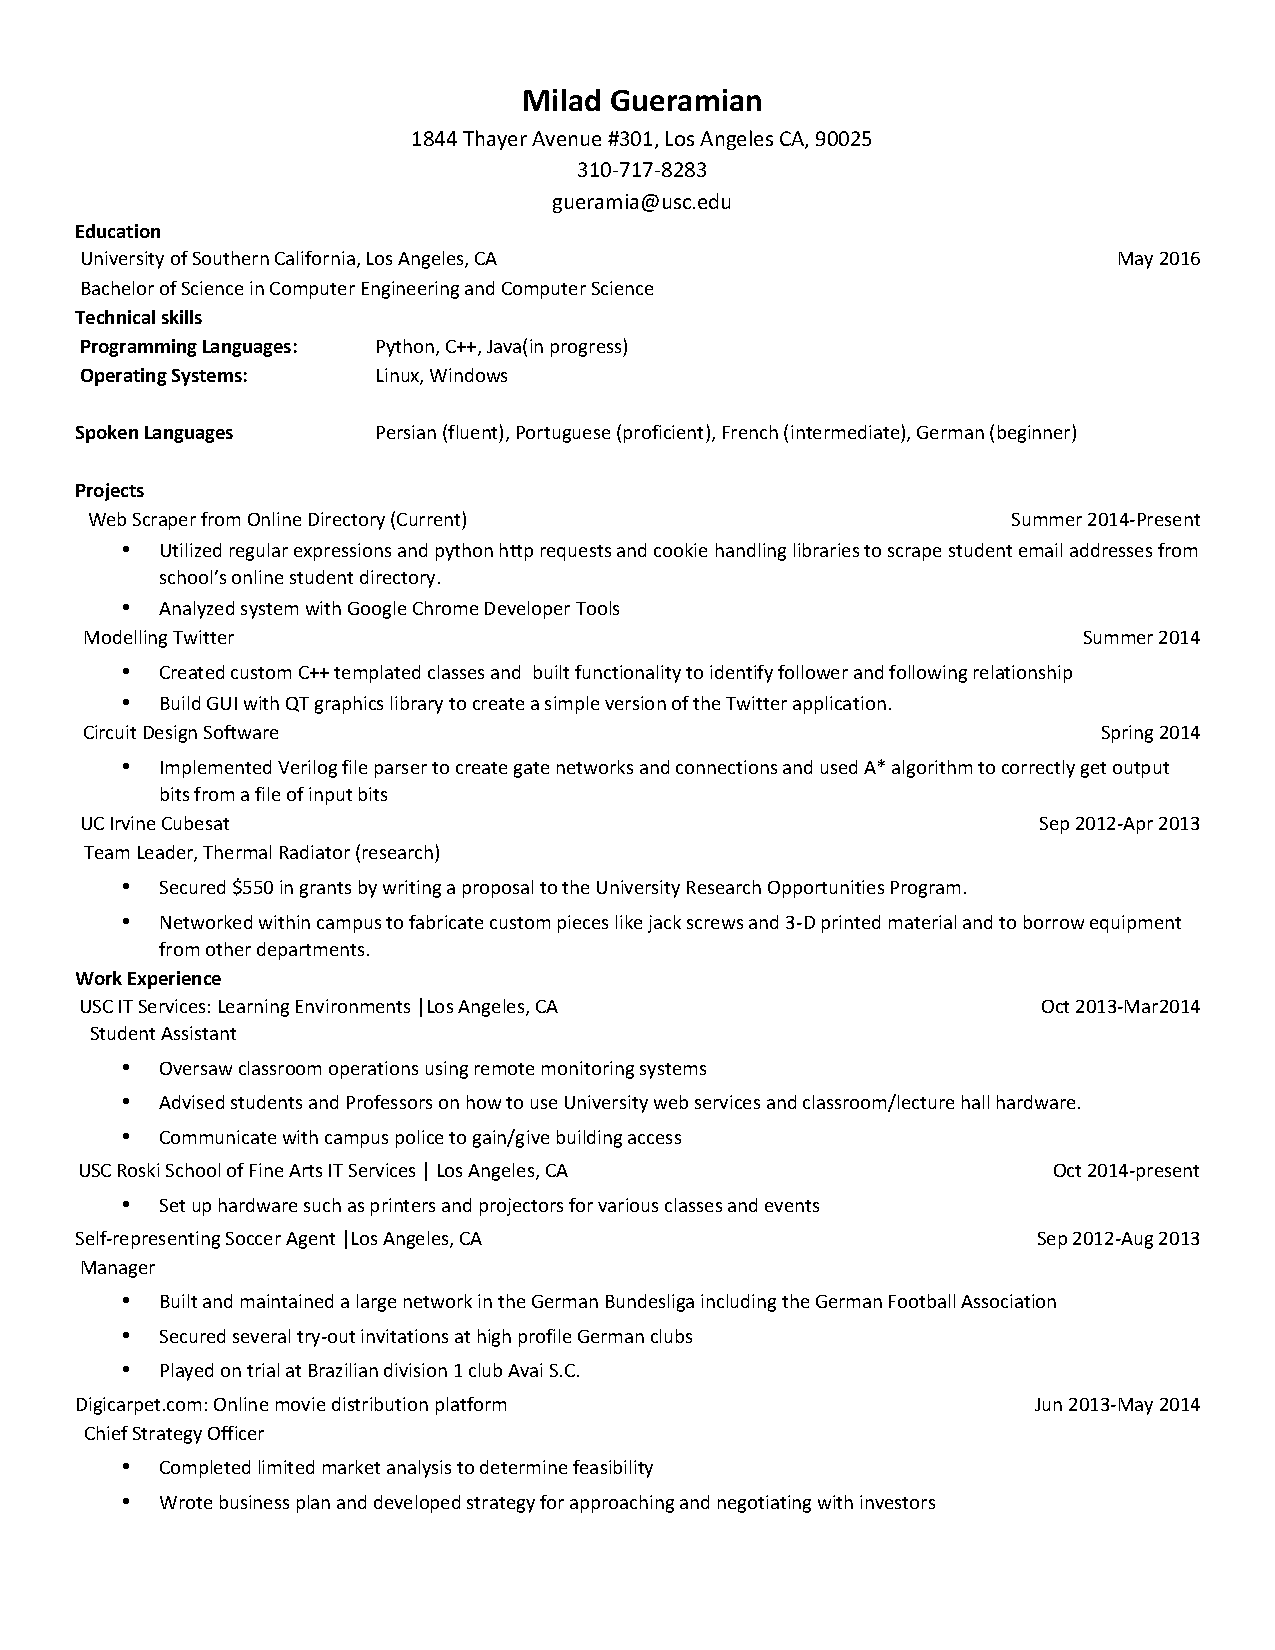
\includegraphics{milad.pdf}
\pagebreak

\pagebreak

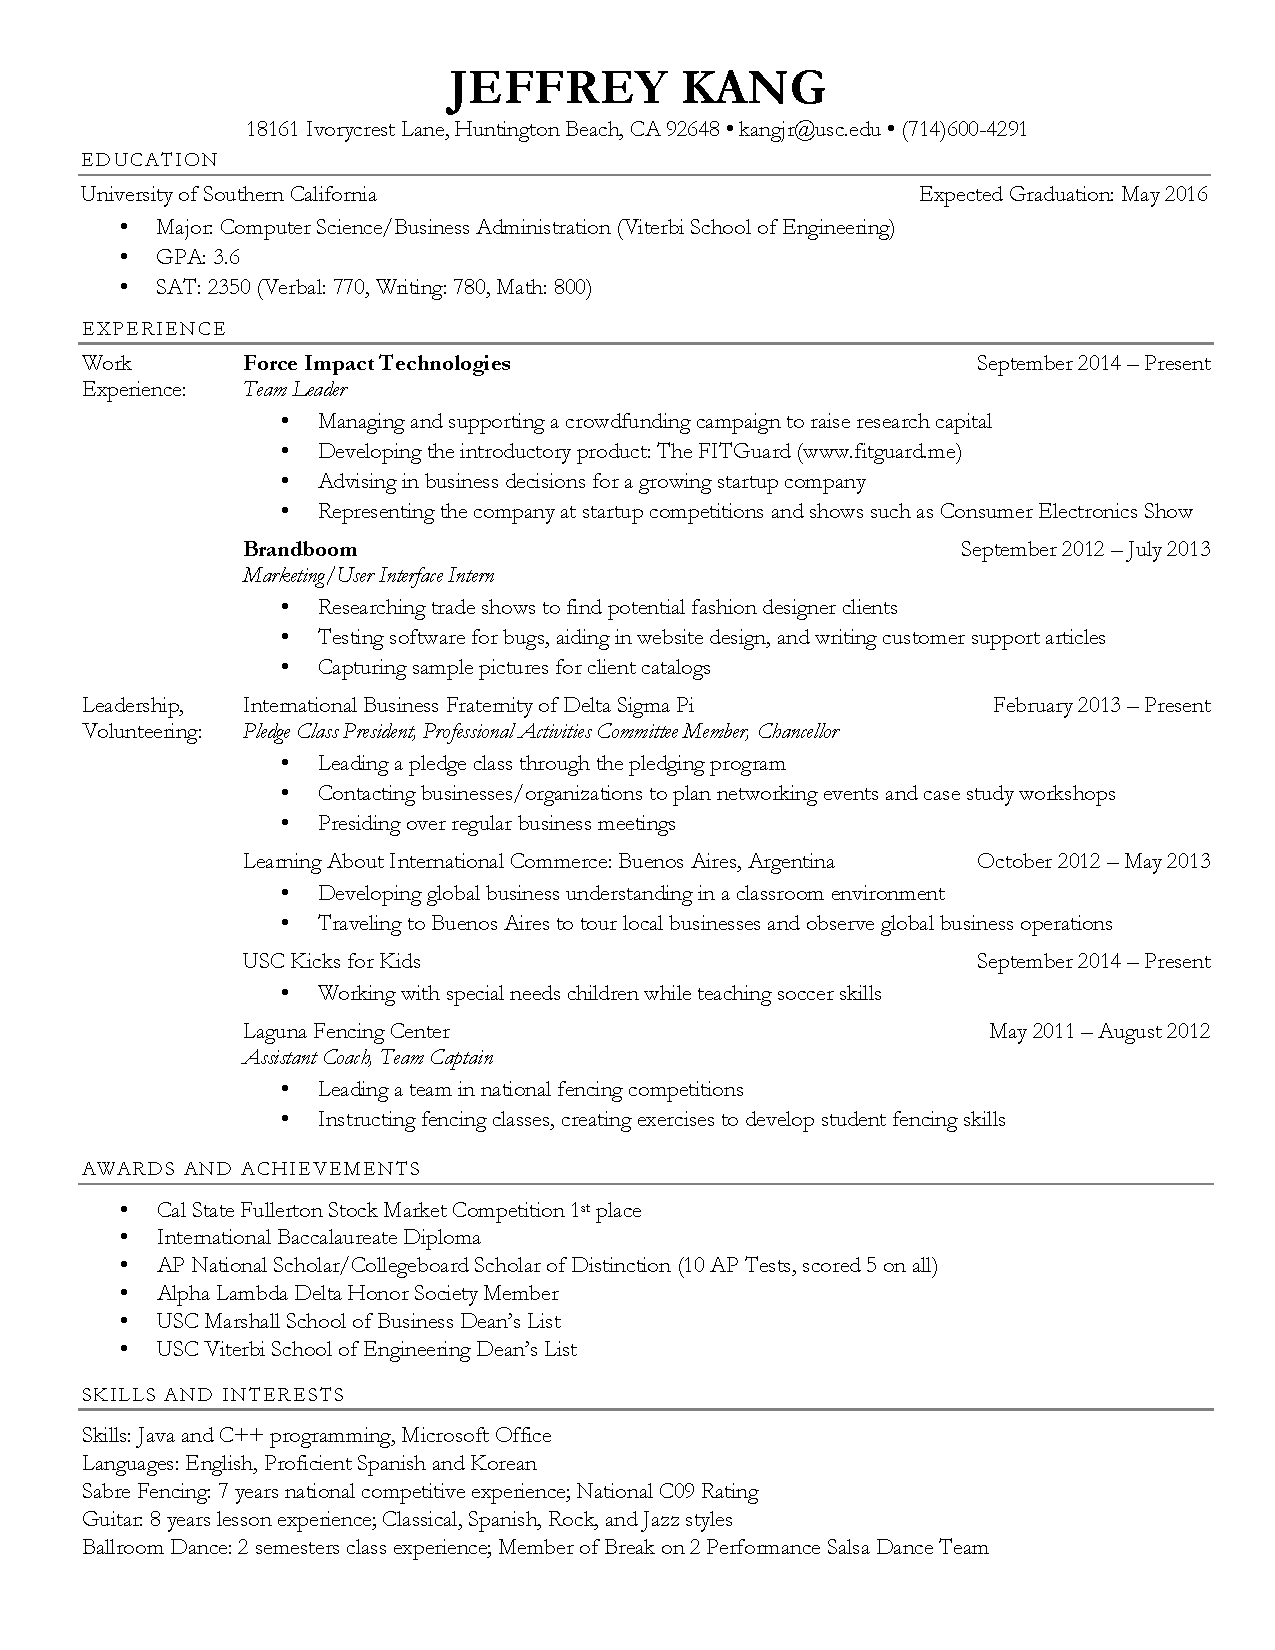
\includegraphics{jeff.pdf}
\pagebreak

\pagebreak

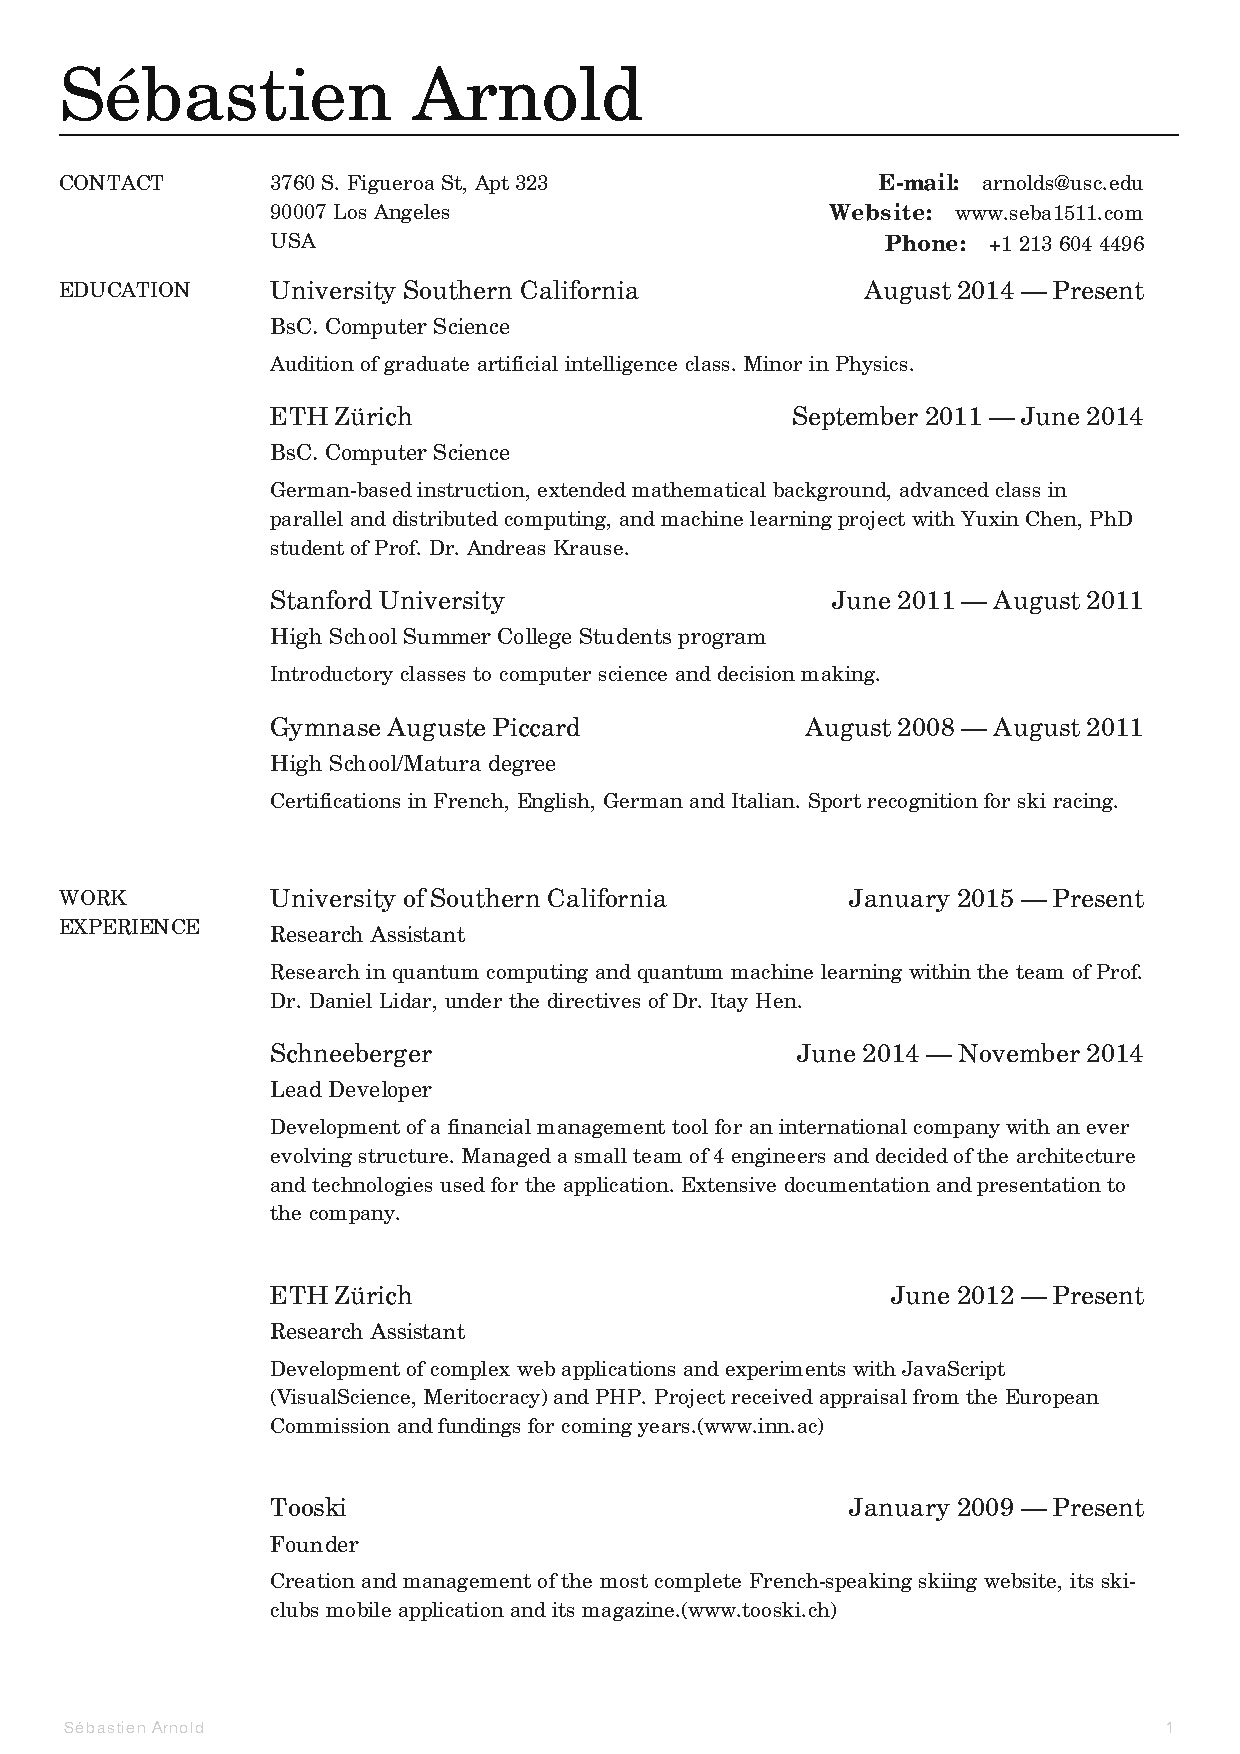
\includegraphics{seb.pdf}
\end{document}
